
% Default to the notebook output style

    


% Inherit from the specified cell style.




    
\documentclass[11pt]{article}

    
    
    \usepackage[T1]{fontenc}
    % Nicer default font (+ math font) than Computer Modern for most use cases
    \usepackage{mathpazo}

    % Basic figure setup, for now with no caption control since it's done
    % automatically by Pandoc (which extracts ![](path) syntax from Markdown).
    \usepackage{graphicx}
    % We will generate all images so they have a width \maxwidth. This means
    % that they will get their normal width if they fit onto the page, but
    % are scaled down if they would overflow the margins.
    \makeatletter
    \def\maxwidth{\ifdim\Gin@nat@width>\linewidth\linewidth
    \else\Gin@nat@width\fi}
    \makeatother
    \let\Oldincludegraphics\includegraphics
    % Set max figure width to be 80% of text width, for now hardcoded.
    \renewcommand{\includegraphics}[1]{\Oldincludegraphics[width=.8\maxwidth]{#1}}
    % Ensure that by default, figures have no caption (until we provide a
    % proper Figure object with a Caption API and a way to capture that
    % in the conversion process - todo).
    \usepackage{caption}
    \DeclareCaptionLabelFormat{nolabel}{}
    \captionsetup{labelformat=nolabel}

    \usepackage{adjustbox} % Used to constrain images to a maximum size 
    \usepackage{xcolor} % Allow colors to be defined
    \usepackage{enumerate} % Needed for markdown enumerations to work
    \usepackage{geometry} % Used to adjust the document margins
    \usepackage{amsmath} % Equations
    \usepackage{amssymb} % Equations
    \usepackage{textcomp} % defines textquotesingle
    % Hack from http://tex.stackexchange.com/a/47451/13684:
    \AtBeginDocument{%
        \def\PYZsq{\textquotesingle}% Upright quotes in Pygmentized code
    }
    \usepackage{upquote} % Upright quotes for verbatim code
    \usepackage{eurosym} % defines \euro
    \usepackage[mathletters]{ucs} % Extended unicode (utf-8) support
    \usepackage[utf8x]{inputenc} % Allow utf-8 characters in the tex document
    \usepackage{fancyvrb} % verbatim replacement that allows latex
    \usepackage{grffile} % extends the file name processing of package graphics 
                         % to support a larger range 
    % The hyperref package gives us a pdf with properly built
    % internal navigation ('pdf bookmarks' for the table of contents,
    % internal cross-reference links, web links for URLs, etc.)
    \usepackage{hyperref}
    \usepackage{longtable} % longtable support required by pandoc >1.10
    \usepackage{booktabs}  % table support for pandoc > 1.12.2
    \usepackage[inline]{enumitem} % IRkernel/repr support (it uses the enumerate* environment)
    \usepackage[normalem]{ulem} % ulem is needed to support strikethroughs (\sout)
                                % normalem makes italics be italics, not underlines
    

    
    
    % Colors for the hyperref package
    \definecolor{urlcolor}{rgb}{0,.145,.698}
    \definecolor{linkcolor}{rgb}{.71,0.21,0.01}
    \definecolor{citecolor}{rgb}{.12,.54,.11}

    % ANSI colors
    \definecolor{ansi-black}{HTML}{3E424D}
    \definecolor{ansi-black-intense}{HTML}{282C36}
    \definecolor{ansi-red}{HTML}{E75C58}
    \definecolor{ansi-red-intense}{HTML}{B22B31}
    \definecolor{ansi-green}{HTML}{00A250}
    \definecolor{ansi-green-intense}{HTML}{007427}
    \definecolor{ansi-yellow}{HTML}{DDB62B}
    \definecolor{ansi-yellow-intense}{HTML}{B27D12}
    \definecolor{ansi-blue}{HTML}{208FFB}
    \definecolor{ansi-blue-intense}{HTML}{0065CA}
    \definecolor{ansi-magenta}{HTML}{D160C4}
    \definecolor{ansi-magenta-intense}{HTML}{A03196}
    \definecolor{ansi-cyan}{HTML}{60C6C8}
    \definecolor{ansi-cyan-intense}{HTML}{258F8F}
    \definecolor{ansi-white}{HTML}{C5C1B4}
    \definecolor{ansi-white-intense}{HTML}{A1A6B2}

    % commands and environments needed by pandoc snippets
    % extracted from the output of `pandoc -s`
    \providecommand{\tightlist}{%
      \setlength{\itemsep}{0pt}\setlength{\parskip}{0pt}}
    \DefineVerbatimEnvironment{Highlighting}{Verbatim}{commandchars=\\\{\}}
    % Add ',fontsize=\small' for more characters per line
    \newenvironment{Shaded}{}{}
    \newcommand{\KeywordTok}[1]{\textcolor[rgb]{0.00,0.44,0.13}{\textbf{{#1}}}}
    \newcommand{\DataTypeTok}[1]{\textcolor[rgb]{0.56,0.13,0.00}{{#1}}}
    \newcommand{\DecValTok}[1]{\textcolor[rgb]{0.25,0.63,0.44}{{#1}}}
    \newcommand{\BaseNTok}[1]{\textcolor[rgb]{0.25,0.63,0.44}{{#1}}}
    \newcommand{\FloatTok}[1]{\textcolor[rgb]{0.25,0.63,0.44}{{#1}}}
    \newcommand{\CharTok}[1]{\textcolor[rgb]{0.25,0.44,0.63}{{#1}}}
    \newcommand{\StringTok}[1]{\textcolor[rgb]{0.25,0.44,0.63}{{#1}}}
    \newcommand{\CommentTok}[1]{\textcolor[rgb]{0.38,0.63,0.69}{\textit{{#1}}}}
    \newcommand{\OtherTok}[1]{\textcolor[rgb]{0.00,0.44,0.13}{{#1}}}
    \newcommand{\AlertTok}[1]{\textcolor[rgb]{1.00,0.00,0.00}{\textbf{{#1}}}}
    \newcommand{\FunctionTok}[1]{\textcolor[rgb]{0.02,0.16,0.49}{{#1}}}
    \newcommand{\RegionMarkerTok}[1]{{#1}}
    \newcommand{\ErrorTok}[1]{\textcolor[rgb]{1.00,0.00,0.00}{\textbf{{#1}}}}
    \newcommand{\NormalTok}[1]{{#1}}
    
    % Additional commands for more recent versions of Pandoc
    \newcommand{\ConstantTok}[1]{\textcolor[rgb]{0.53,0.00,0.00}{{#1}}}
    \newcommand{\SpecialCharTok}[1]{\textcolor[rgb]{0.25,0.44,0.63}{{#1}}}
    \newcommand{\VerbatimStringTok}[1]{\textcolor[rgb]{0.25,0.44,0.63}{{#1}}}
    \newcommand{\SpecialStringTok}[1]{\textcolor[rgb]{0.73,0.40,0.53}{{#1}}}
    \newcommand{\ImportTok}[1]{{#1}}
    \newcommand{\DocumentationTok}[1]{\textcolor[rgb]{0.73,0.13,0.13}{\textit{{#1}}}}
    \newcommand{\AnnotationTok}[1]{\textcolor[rgb]{0.38,0.63,0.69}{\textbf{\textit{{#1}}}}}
    \newcommand{\CommentVarTok}[1]{\textcolor[rgb]{0.38,0.63,0.69}{\textbf{\textit{{#1}}}}}
    \newcommand{\VariableTok}[1]{\textcolor[rgb]{0.10,0.09,0.49}{{#1}}}
    \newcommand{\ControlFlowTok}[1]{\textcolor[rgb]{0.00,0.44,0.13}{\textbf{{#1}}}}
    \newcommand{\OperatorTok}[1]{\textcolor[rgb]{0.40,0.40,0.40}{{#1}}}
    \newcommand{\BuiltInTok}[1]{{#1}}
    \newcommand{\ExtensionTok}[1]{{#1}}
    \newcommand{\PreprocessorTok}[1]{\textcolor[rgb]{0.74,0.48,0.00}{{#1}}}
    \newcommand{\AttributeTok}[1]{\textcolor[rgb]{0.49,0.56,0.16}{{#1}}}
    \newcommand{\InformationTok}[1]{\textcolor[rgb]{0.38,0.63,0.69}{\textbf{\textit{{#1}}}}}
    \newcommand{\WarningTok}[1]{\textcolor[rgb]{0.38,0.63,0.69}{\textbf{\textit{{#1}}}}}
    
    
    % Define a nice break command that doesn't care if a line doesn't already
    % exist.
    \def\br{\hspace*{\fill} \\* }
    % Math Jax compatability definitions
    \def\gt{>}
    \def\lt{<}
    % Document parameters
    \title{project\_2\_starter}
    
    
    

    % Pygments definitions
    
\makeatletter
\def\PY@reset{\let\PY@it=\relax \let\PY@bf=\relax%
    \let\PY@ul=\relax \let\PY@tc=\relax%
    \let\PY@bc=\relax \let\PY@ff=\relax}
\def\PY@tok#1{\csname PY@tok@#1\endcsname}
\def\PY@toks#1+{\ifx\relax#1\empty\else%
    \PY@tok{#1}\expandafter\PY@toks\fi}
\def\PY@do#1{\PY@bc{\PY@tc{\PY@ul{%
    \PY@it{\PY@bf{\PY@ff{#1}}}}}}}
\def\PY#1#2{\PY@reset\PY@toks#1+\relax+\PY@do{#2}}

\expandafter\def\csname PY@tok@w\endcsname{\def\PY@tc##1{\textcolor[rgb]{0.73,0.73,0.73}{##1}}}
\expandafter\def\csname PY@tok@c\endcsname{\let\PY@it=\textit\def\PY@tc##1{\textcolor[rgb]{0.25,0.50,0.50}{##1}}}
\expandafter\def\csname PY@tok@cp\endcsname{\def\PY@tc##1{\textcolor[rgb]{0.74,0.48,0.00}{##1}}}
\expandafter\def\csname PY@tok@k\endcsname{\let\PY@bf=\textbf\def\PY@tc##1{\textcolor[rgb]{0.00,0.50,0.00}{##1}}}
\expandafter\def\csname PY@tok@kp\endcsname{\def\PY@tc##1{\textcolor[rgb]{0.00,0.50,0.00}{##1}}}
\expandafter\def\csname PY@tok@kt\endcsname{\def\PY@tc##1{\textcolor[rgb]{0.69,0.00,0.25}{##1}}}
\expandafter\def\csname PY@tok@o\endcsname{\def\PY@tc##1{\textcolor[rgb]{0.40,0.40,0.40}{##1}}}
\expandafter\def\csname PY@tok@ow\endcsname{\let\PY@bf=\textbf\def\PY@tc##1{\textcolor[rgb]{0.67,0.13,1.00}{##1}}}
\expandafter\def\csname PY@tok@nb\endcsname{\def\PY@tc##1{\textcolor[rgb]{0.00,0.50,0.00}{##1}}}
\expandafter\def\csname PY@tok@nf\endcsname{\def\PY@tc##1{\textcolor[rgb]{0.00,0.00,1.00}{##1}}}
\expandafter\def\csname PY@tok@nc\endcsname{\let\PY@bf=\textbf\def\PY@tc##1{\textcolor[rgb]{0.00,0.00,1.00}{##1}}}
\expandafter\def\csname PY@tok@nn\endcsname{\let\PY@bf=\textbf\def\PY@tc##1{\textcolor[rgb]{0.00,0.00,1.00}{##1}}}
\expandafter\def\csname PY@tok@ne\endcsname{\let\PY@bf=\textbf\def\PY@tc##1{\textcolor[rgb]{0.82,0.25,0.23}{##1}}}
\expandafter\def\csname PY@tok@nv\endcsname{\def\PY@tc##1{\textcolor[rgb]{0.10,0.09,0.49}{##1}}}
\expandafter\def\csname PY@tok@no\endcsname{\def\PY@tc##1{\textcolor[rgb]{0.53,0.00,0.00}{##1}}}
\expandafter\def\csname PY@tok@nl\endcsname{\def\PY@tc##1{\textcolor[rgb]{0.63,0.63,0.00}{##1}}}
\expandafter\def\csname PY@tok@ni\endcsname{\let\PY@bf=\textbf\def\PY@tc##1{\textcolor[rgb]{0.60,0.60,0.60}{##1}}}
\expandafter\def\csname PY@tok@na\endcsname{\def\PY@tc##1{\textcolor[rgb]{0.49,0.56,0.16}{##1}}}
\expandafter\def\csname PY@tok@nt\endcsname{\let\PY@bf=\textbf\def\PY@tc##1{\textcolor[rgb]{0.00,0.50,0.00}{##1}}}
\expandafter\def\csname PY@tok@nd\endcsname{\def\PY@tc##1{\textcolor[rgb]{0.67,0.13,1.00}{##1}}}
\expandafter\def\csname PY@tok@s\endcsname{\def\PY@tc##1{\textcolor[rgb]{0.73,0.13,0.13}{##1}}}
\expandafter\def\csname PY@tok@sd\endcsname{\let\PY@it=\textit\def\PY@tc##1{\textcolor[rgb]{0.73,0.13,0.13}{##1}}}
\expandafter\def\csname PY@tok@si\endcsname{\let\PY@bf=\textbf\def\PY@tc##1{\textcolor[rgb]{0.73,0.40,0.53}{##1}}}
\expandafter\def\csname PY@tok@se\endcsname{\let\PY@bf=\textbf\def\PY@tc##1{\textcolor[rgb]{0.73,0.40,0.13}{##1}}}
\expandafter\def\csname PY@tok@sr\endcsname{\def\PY@tc##1{\textcolor[rgb]{0.73,0.40,0.53}{##1}}}
\expandafter\def\csname PY@tok@ss\endcsname{\def\PY@tc##1{\textcolor[rgb]{0.10,0.09,0.49}{##1}}}
\expandafter\def\csname PY@tok@sx\endcsname{\def\PY@tc##1{\textcolor[rgb]{0.00,0.50,0.00}{##1}}}
\expandafter\def\csname PY@tok@m\endcsname{\def\PY@tc##1{\textcolor[rgb]{0.40,0.40,0.40}{##1}}}
\expandafter\def\csname PY@tok@gh\endcsname{\let\PY@bf=\textbf\def\PY@tc##1{\textcolor[rgb]{0.00,0.00,0.50}{##1}}}
\expandafter\def\csname PY@tok@gu\endcsname{\let\PY@bf=\textbf\def\PY@tc##1{\textcolor[rgb]{0.50,0.00,0.50}{##1}}}
\expandafter\def\csname PY@tok@gd\endcsname{\def\PY@tc##1{\textcolor[rgb]{0.63,0.00,0.00}{##1}}}
\expandafter\def\csname PY@tok@gi\endcsname{\def\PY@tc##1{\textcolor[rgb]{0.00,0.63,0.00}{##1}}}
\expandafter\def\csname PY@tok@gr\endcsname{\def\PY@tc##1{\textcolor[rgb]{1.00,0.00,0.00}{##1}}}
\expandafter\def\csname PY@tok@ge\endcsname{\let\PY@it=\textit}
\expandafter\def\csname PY@tok@gs\endcsname{\let\PY@bf=\textbf}
\expandafter\def\csname PY@tok@gp\endcsname{\let\PY@bf=\textbf\def\PY@tc##1{\textcolor[rgb]{0.00,0.00,0.50}{##1}}}
\expandafter\def\csname PY@tok@go\endcsname{\def\PY@tc##1{\textcolor[rgb]{0.53,0.53,0.53}{##1}}}
\expandafter\def\csname PY@tok@gt\endcsname{\def\PY@tc##1{\textcolor[rgb]{0.00,0.27,0.87}{##1}}}
\expandafter\def\csname PY@tok@err\endcsname{\def\PY@bc##1{\setlength{\fboxsep}{0pt}\fcolorbox[rgb]{1.00,0.00,0.00}{1,1,1}{\strut ##1}}}
\expandafter\def\csname PY@tok@kc\endcsname{\let\PY@bf=\textbf\def\PY@tc##1{\textcolor[rgb]{0.00,0.50,0.00}{##1}}}
\expandafter\def\csname PY@tok@kd\endcsname{\let\PY@bf=\textbf\def\PY@tc##1{\textcolor[rgb]{0.00,0.50,0.00}{##1}}}
\expandafter\def\csname PY@tok@kn\endcsname{\let\PY@bf=\textbf\def\PY@tc##1{\textcolor[rgb]{0.00,0.50,0.00}{##1}}}
\expandafter\def\csname PY@tok@kr\endcsname{\let\PY@bf=\textbf\def\PY@tc##1{\textcolor[rgb]{0.00,0.50,0.00}{##1}}}
\expandafter\def\csname PY@tok@bp\endcsname{\def\PY@tc##1{\textcolor[rgb]{0.00,0.50,0.00}{##1}}}
\expandafter\def\csname PY@tok@fm\endcsname{\def\PY@tc##1{\textcolor[rgb]{0.00,0.00,1.00}{##1}}}
\expandafter\def\csname PY@tok@vc\endcsname{\def\PY@tc##1{\textcolor[rgb]{0.10,0.09,0.49}{##1}}}
\expandafter\def\csname PY@tok@vg\endcsname{\def\PY@tc##1{\textcolor[rgb]{0.10,0.09,0.49}{##1}}}
\expandafter\def\csname PY@tok@vi\endcsname{\def\PY@tc##1{\textcolor[rgb]{0.10,0.09,0.49}{##1}}}
\expandafter\def\csname PY@tok@vm\endcsname{\def\PY@tc##1{\textcolor[rgb]{0.10,0.09,0.49}{##1}}}
\expandafter\def\csname PY@tok@sa\endcsname{\def\PY@tc##1{\textcolor[rgb]{0.73,0.13,0.13}{##1}}}
\expandafter\def\csname PY@tok@sb\endcsname{\def\PY@tc##1{\textcolor[rgb]{0.73,0.13,0.13}{##1}}}
\expandafter\def\csname PY@tok@sc\endcsname{\def\PY@tc##1{\textcolor[rgb]{0.73,0.13,0.13}{##1}}}
\expandafter\def\csname PY@tok@dl\endcsname{\def\PY@tc##1{\textcolor[rgb]{0.73,0.13,0.13}{##1}}}
\expandafter\def\csname PY@tok@s2\endcsname{\def\PY@tc##1{\textcolor[rgb]{0.73,0.13,0.13}{##1}}}
\expandafter\def\csname PY@tok@sh\endcsname{\def\PY@tc##1{\textcolor[rgb]{0.73,0.13,0.13}{##1}}}
\expandafter\def\csname PY@tok@s1\endcsname{\def\PY@tc##1{\textcolor[rgb]{0.73,0.13,0.13}{##1}}}
\expandafter\def\csname PY@tok@mb\endcsname{\def\PY@tc##1{\textcolor[rgb]{0.40,0.40,0.40}{##1}}}
\expandafter\def\csname PY@tok@mf\endcsname{\def\PY@tc##1{\textcolor[rgb]{0.40,0.40,0.40}{##1}}}
\expandafter\def\csname PY@tok@mh\endcsname{\def\PY@tc##1{\textcolor[rgb]{0.40,0.40,0.40}{##1}}}
\expandafter\def\csname PY@tok@mi\endcsname{\def\PY@tc##1{\textcolor[rgb]{0.40,0.40,0.40}{##1}}}
\expandafter\def\csname PY@tok@il\endcsname{\def\PY@tc##1{\textcolor[rgb]{0.40,0.40,0.40}{##1}}}
\expandafter\def\csname PY@tok@mo\endcsname{\def\PY@tc##1{\textcolor[rgb]{0.40,0.40,0.40}{##1}}}
\expandafter\def\csname PY@tok@ch\endcsname{\let\PY@it=\textit\def\PY@tc##1{\textcolor[rgb]{0.25,0.50,0.50}{##1}}}
\expandafter\def\csname PY@tok@cm\endcsname{\let\PY@it=\textit\def\PY@tc##1{\textcolor[rgb]{0.25,0.50,0.50}{##1}}}
\expandafter\def\csname PY@tok@cpf\endcsname{\let\PY@it=\textit\def\PY@tc##1{\textcolor[rgb]{0.25,0.50,0.50}{##1}}}
\expandafter\def\csname PY@tok@c1\endcsname{\let\PY@it=\textit\def\PY@tc##1{\textcolor[rgb]{0.25,0.50,0.50}{##1}}}
\expandafter\def\csname PY@tok@cs\endcsname{\let\PY@it=\textit\def\PY@tc##1{\textcolor[rgb]{0.25,0.50,0.50}{##1}}}

\def\PYZbs{\char`\\}
\def\PYZus{\char`\_}
\def\PYZob{\char`\{}
\def\PYZcb{\char`\}}
\def\PYZca{\char`\^}
\def\PYZam{\char`\&}
\def\PYZlt{\char`\<}
\def\PYZgt{\char`\>}
\def\PYZsh{\char`\#}
\def\PYZpc{\char`\%}
\def\PYZdl{\char`\$}
\def\PYZhy{\char`\-}
\def\PYZsq{\char`\'}
\def\PYZdq{\char`\"}
\def\PYZti{\char`\~}
% for compatibility with earlier versions
\def\PYZat{@}
\def\PYZlb{[}
\def\PYZrb{]}
\makeatother


    % Exact colors from NB
    \definecolor{incolor}{rgb}{0.0, 0.0, 0.5}
    \definecolor{outcolor}{rgb}{0.545, 0.0, 0.0}



    
    % Prevent overflowing lines due to hard-to-break entities
    \sloppy 
    % Setup hyperref package
    \hypersetup{
      breaklinks=true,  % so long urls are correctly broken across lines
      colorlinks=true,
      urlcolor=urlcolor,
      linkcolor=linkcolor,
      citecolor=citecolor,
      }
    % Slightly bigger margins than the latex defaults
    
    \geometry{verbose,tmargin=1in,bmargin=1in,lmargin=1in,rmargin=1in}
    
    

    \begin{document}
    
    
    \maketitle
    
    

    
    \hypertarget{project-2-breakout-strategy}{%
\section{Project 2: Breakout
Strategy}\label{project-2-breakout-strategy}}

\hypertarget{instructions}{%
\subsection{Instructions}\label{instructions}}

Each problem consists of a function to implement and instructions on how
to implement the function. The parts of the function that need to be
implemented are marked with a \texttt{\#\ TODO} comment. After
implementing the function, run the cell to test it against the unit
tests we've provided. For each problem, we provide one or more unit
tests from our \texttt{project\_tests} package. These unit tests won't
tell you if your answer is correct, but will warn you of any major
errors. Your code will be checked for the correct solution when you
submit it to Udacity.

\hypertarget{packages}{%
\subsection{Packages}\label{packages}}

When you implement the functions, you'll only need to you use the
packages you've used in the classroom, like
\href{https://pandas.pydata.org/}{Pandas} and
\href{http://www.numpy.org/}{Numpy}. These packages will be imported for
you. We recommend you don't add any import statements, otherwise the
grader might not be able to run your code.

The other packages that we're importing are \texttt{helper},
\texttt{project\_helper}, and \texttt{project\_tests}. These are custom
packages built to help you solve the problems. The \texttt{helper} and
\texttt{project\_helper} module contains utility functions and graph
functions. The \texttt{project\_tests} contains the unit tests for all
the problems.

\hypertarget{install-packages}{%
\subsubsection{Install Packages}\label{install-packages}}

    \begin{Verbatim}[commandchars=\\\{\}]
{\color{incolor}In [{\color{incolor}1}]:} \PY{k+kn}{import} \PY{n+nn}{sys}
        \PY{o}{!}\PY{o}{\PYZob{}}sys.executable\PY{o}{\PYZcb{}} \PYZhy{}m pip install \PYZhy{}r requirements.txt
\end{Verbatim}


    \begin{Verbatim}[commandchars=\\\{\}]
Requirement already satisfied: colour==0.1.5 in /opt/conda/lib/python3.6/site-packages (from -r requirements.txt (line 1))
Collecting cvxpy==1.0.3 (from -r requirements.txt (line 2))
  Downloading https://files.pythonhosted.org/packages/a1/59/2613468ffbbe3a818934d06b81b9f4877fe054afbf4f99d2f43f398a0b34/cvxpy-1.0.3.tar.gz (880kB)
    100\% |████████████████████████████████| 880kB 645kB/s ta 0:00:01    65\% |████████████████████▉           | 573kB 6.6MB/s eta 0:00:01
Requirement already satisfied: cycler==0.10.0 in /opt/conda/lib/python3.6/site-packages/cycler-0.10.0-py3.6.egg (from -r requirements.txt (line 3))
Collecting numpy==1.13.3 (from -r requirements.txt (line 4))
  Downloading https://files.pythonhosted.org/packages/57/a7/e3e6bd9d595125e1abbe162e323fd2d06f6f6683185294b79cd2cdb190d5/numpy-1.13.3-cp36-cp36m-manylinux1\_x86\_64.whl (17.0MB)
    100\% |████████████████████████████████| 17.0MB 37kB/s  eta 0:00:01   10\% |███▎                            | 1.8MB 19.4MB/s eta 0:00:01    39\% |████████████▌                   | 6.6MB 31.4MB/s eta 0:00:01    64\% |████████████████████▊           | 11.0MB 34.9MB/s eta 0:00:01
Collecting pandas==0.21.1 (from -r requirements.txt (line 5))
  Downloading https://files.pythonhosted.org/packages/3a/e1/6c514df670b887c77838ab856f57783c07e8760f2e3d5939203a39735e0e/pandas-0.21.1-cp36-cp36m-manylinux1\_x86\_64.whl (26.2MB)
    100\% |████████████████████████████████| 26.2MB 23kB/s  eta 0:00:01  9\% |███▏                            | 2.6MB 29.0MB/s eta 0:00:01    36\% |███████████▋                    | 9.5MB 29.0MB/s eta 0:00:01    76\% |████████████████████████▌       | 20.1MB 25.5MB/s eta 0:00:01    89\% |████████████████████████████▋   | 23.5MB 25.1MB/s eta 0:00:01    94\% |██████████████████████████████▏ | 24.7MB 23.0MB/s eta 0:00:01
Collecting plotly==2.2.3 (from -r requirements.txt (line 6))
  Downloading https://files.pythonhosted.org/packages/99/a6/8214b6564bf4ace9bec8a26e7f89832792be582c042c47c912d3201328a0/plotly-2.2.3.tar.gz (1.1MB)
    100\% |████████████████████████████████| 1.1MB 589kB/s eta 0:00:01
Requirement already satisfied: pyparsing==2.2.0 in /opt/conda/lib/python3.6/site-packages (from -r requirements.txt (line 7))
Requirement already satisfied: python-dateutil==2.6.1 in /opt/conda/lib/python3.6/site-packages (from -r requirements.txt (line 8))
Requirement already satisfied: pytz==2017.3 in /opt/conda/lib/python3.6/site-packages (from -r requirements.txt (line 9))
Requirement already satisfied: requests==2.18.4 in /opt/conda/lib/python3.6/site-packages (from -r requirements.txt (line 10))
Collecting scipy==1.0.0 (from -r requirements.txt (line 11))
  Downloading https://files.pythonhosted.org/packages/d8/5e/caa01ba7be11600b6a9d39265440d7b3be3d69206da887c42bef049521f2/scipy-1.0.0-cp36-cp36m-manylinux1\_x86\_64.whl (50.0MB)
    100\% |████████████████████████████████| 50.0MB 12kB/s  eta 0:00:01  3\% |█                               | 1.6MB 25.8MB/s eta 0:00:02    5\% |█▊                              | 2.8MB 23.0MB/s eta 0:00:03    9\% |███▏                            | 4.9MB 21.9MB/s eta 0:00:03    20\% |██████▌                         | 10.2MB 22.1MB/s eta 0:00:02    29\% |█████████▎                      | 14.6MB 19.2MB/s eta 0:00:02    33\% |██████████▊                     | 16.7MB 23.9MB/s eta 0:00:02    37\% |████████████                    | 18.9MB 24.6MB/s eta 0:00:02    40\% |████████████▉                   | 20.1MB 24.0MB/s eta 0:00:02    44\% |██████████████▎                 | 22.3MB 25.1MB/s eta 0:00:02    51\% |████████████████▍               | 25.6MB 22.9MB/s eta 0:00:02    53\% |█████████████████               | 26.6MB 24.9MB/s eta 0:00:01    55\% |█████████████████▉              | 27.8MB 21.8MB/s eta 0:00:02    57\% |██████████████████▌             | 28.9MB 24.1MB/s eta 0:00:01    60\% |███████████████████▎            | 30.1MB 25.7MB/s eta 0:00:01    66\% |█████████████████████▍          | 33.4MB 22.3MB/s eta 0:00:01    68\% |██████████████████████          | 34.5MB 23.4MB/s eta 0:00:01    71\% |██████████████████████▉         | 35.6MB 33.2MB/s eta 0:00:01    75\% |████████████████████████▎       | 37.9MB 22.9MB/s eta 0:00:01    77\% |█████████████████████████       | 39.0MB 24.7MB/s eta 0:00:01    80\% |█████████████████████████▊      | 40.2MB 25.9MB/s eta 0:00:01    82\% |██████████████████████████▌     | 41.4MB 30.0MB/s eta 0:00:01    87\% |████████████████████████████    | 43.7MB 24.6MB/s eta 0:00:01    89\% |████████████████████████████▊   | 44.8MB 22.3MB/s eta 0:00:01    91\% |█████████████████████████████▍  | 45.9MB 24.6MB/s eta 0:00:01    94\% |██████████████████████████████  | 47.0MB 21.8MB/s eta 0:00:01    96\% |██████████████████████████████▉ | 48.1MB 28.2MB/s eta 0:00:01
Requirement already satisfied: scikit-learn==0.19.1 in /opt/conda/lib/python3.6/site-packages (from -r requirements.txt (line 12))
Requirement already satisfied: six==1.11.0 in /opt/conda/lib/python3.6/site-packages (from -r requirements.txt (line 13))
Collecting tqdm==4.19.5 (from -r requirements.txt (line 14))
  Downloading https://files.pythonhosted.org/packages/71/3c/341b4fa23cb3abc335207dba057c790f3bb329f6757e1fcd5d347bcf8308/tqdm-4.19.5-py2.py3-none-any.whl (51kB)
    100\% |████████████████████████████████| 61kB 3.7MB/s eta 0:00:01
Collecting zipline==1.2.0 (from -r requirements.txt (line 15))
  Downloading https://files.pythonhosted.org/packages/15/d3/689f2a940478b82ac57c751a40460598221fd82b0449a7a8f7eef47a3bcc/zipline-1.2.0.tar.gz (659kB)
    100\% |████████████████████████████████| 665kB 921kB/s eta 0:00:01    29\% |█████████▍                      | 194kB 24.7MB/s eta 0:00:01
Collecting osqp (from cvxpy==1.0.3->-r requirements.txt (line 2))
  Downloading https://files.pythonhosted.org/packages/05/42/0ccab82eb6ed0edb83d184928ec864232dc00c3cf968a4b92a02caf0f7ec/osqp-0.4.0-cp36-cp36m-manylinux1\_x86\_64.whl (146kB)
    100\% |████████████████████████████████| 153kB 3.6MB/s eta 0:00:01
Collecting ecos>=2 (from cvxpy==1.0.3->-r requirements.txt (line 2))
  Downloading https://files.pythonhosted.org/packages/b6/b4/988b15513b13e8ea2eac65e97d84221ac515a735a93f046e2a2a3d7863fc/ecos-2.0.5.tar.gz (114kB)
    100\% |████████████████████████████████| 122kB 3.7MB/s eta 0:00:01
Collecting scs>=1.1.3 (from cvxpy==1.0.3->-r requirements.txt (line 2))
  Downloading https://files.pythonhosted.org/packages/b3/fd/6e01c4f4a69fcc6c3db130ba55572089e78e77ea8c0921a679f9da1ec04c/scs-2.0.2.tar.gz (133kB)
    100\% |████████████████████████████████| 143kB 3.4MB/s eta 0:00:01
Collecting multiprocess (from cvxpy==1.0.3->-r requirements.txt (line 2))
  Downloading https://files.pythonhosted.org/packages/7a/ee/b9bf3e171f936743758ef924622d8dd00516c5532b00a1210a09bce68325/multiprocess-0.70.6.1.tar.gz (1.4MB)
    100\% |████████████████████████████████| 1.4MB 447kB/s eta 0:00:01
Requirement already satisfied: fastcache in /opt/conda/lib/python3.6/site-packages (from cvxpy==1.0.3->-r requirements.txt (line 2))
Requirement already satisfied: toolz in /opt/conda/lib/python3.6/site-packages (from cvxpy==1.0.3->-r requirements.txt (line 2))
Requirement already satisfied: decorator>=4.0.6 in /opt/conda/lib/python3.6/site-packages (from plotly==2.2.3->-r requirements.txt (line 6))
Requirement already satisfied: nbformat>=4.2 in /opt/conda/lib/python3.6/site-packages (from plotly==2.2.3->-r requirements.txt (line 6))
Requirement already satisfied: chardet<3.1.0,>=3.0.2 in /opt/conda/lib/python3.6/site-packages (from requests==2.18.4->-r requirements.txt (line 10))
Requirement already satisfied: idna<2.7,>=2.5 in /opt/conda/lib/python3.6/site-packages (from requests==2.18.4->-r requirements.txt (line 10))
Requirement already satisfied: urllib3<1.23,>=1.21.1 in /opt/conda/lib/python3.6/site-packages (from requests==2.18.4->-r requirements.txt (line 10))
Requirement already satisfied: certifi>=2017.4.17 in /opt/conda/lib/python3.6/site-packages (from requests==2.18.4->-r requirements.txt (line 10))
Requirement already satisfied: pip>=7.1.0 in /opt/conda/lib/python3.6/site-packages (from zipline==1.2.0->-r requirements.txt (line 15))
Requirement already satisfied: setuptools>18.0 in /opt/conda/lib/python3.6/site-packages (from zipline==1.2.0->-r requirements.txt (line 15))
Collecting Logbook>=0.12.5 (from zipline==1.2.0->-r requirements.txt (line 15))
  Downloading https://files.pythonhosted.org/packages/36/4b/b610bee18d5cfc4cec7dde056639994e9b34991e4c57816bfff0f3d0ac33/Logbook-1.4.0.tar.gz (84kB)
    100\% |████████████████████████████████| 92kB 4.4MB/s eta 0:00:01
Collecting requests-file>=1.4.1 (from zipline==1.2.0->-r requirements.txt (line 15))
  Downloading https://files.pythonhosted.org/packages/23/9c/6e63c23c39e53d3df41c77a3d05a49a42c4e1383a6d2a5e3233161b89dbf/requests\_file-1.4.3-py2.py3-none-any.whl
Collecting pandas-datareader<0.6,>=0.2.1 (from zipline==1.2.0->-r requirements.txt (line 15))
  Downloading https://files.pythonhosted.org/packages/40/c5/cc720f531bbde0efeab940de400d0fcc95e87770a3abcd7f90d6d52a3302/pandas\_datareader-0.5.0-py2.py3-none-any.whl (74kB)
    100\% |████████████████████████████████| 81kB 4.0MB/s eta 0:00:01
Requirement already satisfied: patsy>=0.4.0 in /opt/conda/lib/python3.6/site-packages (from zipline==1.2.0->-r requirements.txt (line 15))
Requirement already satisfied: statsmodels>=0.6.1 in /opt/conda/lib/python3.6/site-packages (from zipline==1.2.0->-r requirements.txt (line 15))
Requirement already satisfied: Cython>=0.25.2 in /opt/conda/lib/python3.6/site-packages (from zipline==1.2.0->-r requirements.txt (line 15))
Collecting cyordereddict>=0.2.2 (from zipline==1.2.0->-r requirements.txt (line 15))
  Downloading https://files.pythonhosted.org/packages/d1/1a/364cbfd927be1b743c7f0a985a7f1f7e8a51469619f9fefe4ee9240ba210/cyordereddict-1.0.0.tar.gz (138kB)
    100\% |████████████████████████████████| 143kB 3.5MB/s eta 0:00:01
Collecting bottleneck>=1.0.0 (from zipline==1.2.0->-r requirements.txt (line 15))
  Downloading https://files.pythonhosted.org/packages/05/ae/cedf5323f398ab4e4ff92d6c431a3e1c6a186f9b41ab3e8258dff786a290/Bottleneck-1.2.1.tar.gz (105kB)
    100\% |████████████████████████████████| 112kB 3.8MB/s eta 0:00:01
Collecting contextlib2>=0.4.0 (from zipline==1.2.0->-r requirements.txt (line 15))
  Downloading https://files.pythonhosted.org/packages/a2/71/8273a7eeed0aff6a854237ab5453bc9aa67deb49df4832801c21f0ff3782/contextlib2-0.5.5-py2.py3-none-any.whl
Requirement already satisfied: networkx<2.0,>=1.9.1 in /opt/conda/lib/python3.6/site-packages (from zipline==1.2.0->-r requirements.txt (line 15))
Requirement already satisfied: numexpr>=2.6.1 in /opt/conda/lib/python3.6/site-packages (from zipline==1.2.0->-r requirements.txt (line 15))
Collecting bcolz<1,>=0.12.1 (from zipline==1.2.0->-r requirements.txt (line 15))
  Downloading https://files.pythonhosted.org/packages/6c/8b/1ffa01f872cac36173c5eb95b58c01040d8d25f1b242c48577f4104cd3ab/bcolz-0.12.1.tar.gz (622kB)
    100\% |████████████████████████████████| 624kB 965kB/s eta 0:00:01
Requirement already satisfied: click>=4.0.0 in /opt/conda/lib/python3.6/site-packages (from zipline==1.2.0->-r requirements.txt (line 15))
Collecting multipledispatch>=0.4.8 (from zipline==1.2.0->-r requirements.txt (line 15))
  Downloading https://files.pythonhosted.org/packages/89/79/429ecef45fd5e4504f7474d4c3c3c4668c267be3370e4c2fd33e61506833/multipledispatch-0.6.0-py3-none-any.whl
Requirement already satisfied: MarkupSafe>=0.23 in /opt/conda/lib/python3.6/site-packages (from zipline==1.2.0->-r requirements.txt (line 15))
Requirement already satisfied: Mako>=1.0.1 in /opt/conda/lib/python3.6/site-packages/Mako-1.0.7-py3.6.egg (from zipline==1.2.0->-r requirements.txt (line 15))
Requirement already satisfied: sqlalchemy>=1.0.8 in /opt/conda/lib/python3.6/site-packages (from zipline==1.2.0->-r requirements.txt (line 15))
Collecting alembic>=0.7.7 (from zipline==1.2.0->-r requirements.txt (line 15))
  Downloading https://files.pythonhosted.org/packages/96/c7/a4129db460c3e0ea8fea0c9eb5de6680d38ea6b6dcffcb88898ae42e170a/alembic-1.0.0-py2.py3-none-any.whl (158kB)
    100\% |████████████████████████████████| 163kB 3.5MB/s eta 0:00:01
Collecting sortedcontainers>=1.4.4 (from zipline==1.2.0->-r requirements.txt (line 15))
  Downloading https://files.pythonhosted.org/packages/be/e3/a065de5fdd5849450a8a16a52a96c8db5f498f245e7eda06cc6725d04b80/sortedcontainers-2.0.5-py2.py3-none-any.whl
Collecting intervaltree>=2.1.0 (from zipline==1.2.0->-r requirements.txt (line 15))
  Downloading https://files.pythonhosted.org/packages/ca/c1/450d109b70fa58ca9d77972b02f69222412f9175ccf99fdeaf167be9583c/intervaltree-2.1.0.tar.gz
Collecting lru-dict>=1.1.4 (from zipline==1.2.0->-r requirements.txt (line 15))
  Downloading https://files.pythonhosted.org/packages/00/a5/32ed6e10246cd341ca8cc205acea5d208e4053f48a4dced2b1b31d45ba3f/lru-dict-1.1.6.tar.gz
Collecting empyrical>=0.4.2 (from zipline==1.2.0->-r requirements.txt (line 15))
  Downloading https://files.pythonhosted.org/packages/7b/55/a01b05162b764830dbbac868462f44cd847a5b6523a01ca9f955721819da/empyrical-0.5.0.tar.gz (49kB)
    100\% |████████████████████████████████| 51kB 3.2MB/s ta 0:00:01
Collecting tables>=3.3.0 (from zipline==1.2.0->-r requirements.txt (line 15))
  Downloading https://files.pythonhosted.org/packages/d7/1b/21f4c7f296b718575c17ef25e61c05742a283c45077b4c8d5a190b3e0b59/tables-3.4.4-cp36-cp36m-manylinux1\_x86\_64.whl (3.8MB)
    100\% |████████████████████████████████| 3.8MB 169kB/s eta 0:00:01
Requirement already satisfied: future in /opt/conda/lib/python3.6/site-packages (from osqp->cvxpy==1.0.3->-r requirements.txt (line 2))
Collecting dill>=0.2.8.1 (from multiprocess->cvxpy==1.0.3->-r requirements.txt (line 2))
  Downloading https://files.pythonhosted.org/packages/6f/78/8b96476f4ae426db71c6e86a8e6a81407f015b34547e442291cd397b18f3/dill-0.2.8.2.tar.gz (150kB)
    100\% |████████████████████████████████| 153kB 3.2MB/s eta 0:00:01
Requirement already satisfied: traitlets>=4.1 in /opt/conda/lib/python3.6/site-packages (from nbformat>=4.2->plotly==2.2.3->-r requirements.txt (line 6))
Requirement already satisfied: jsonschema!=2.5.0,>=2.4 in /opt/conda/lib/python3.6/site-packages (from nbformat>=4.2->plotly==2.2.3->-r requirements.txt (line 6))
Requirement already satisfied: ipython-genutils in /opt/conda/lib/python3.6/site-packages (from nbformat>=4.2->plotly==2.2.3->-r requirements.txt (line 6))
Requirement already satisfied: jupyter-core in /opt/conda/lib/python3.6/site-packages (from nbformat>=4.2->plotly==2.2.3->-r requirements.txt (line 6))
Collecting requests-ftp (from pandas-datareader<0.6,>=0.2.1->zipline==1.2.0->-r requirements.txt (line 15))
  Downloading https://files.pythonhosted.org/packages/3d/ca/14b2ad1e93b5195eeaf56b86b7ecfd5ea2d5754a68d17aeb1e5b9f95b3cf/requests-ftp-0.3.1.tar.gz
Collecting python-editor>=0.3 (from alembic>=0.7.7->zipline==1.2.0->-r requirements.txt (line 15))
  Downloading https://files.pythonhosted.org/packages/65/1e/adf6e000ea5dc909aa420352d6ba37f16434c8a3c2fa030445411a1ed545/python-editor-1.0.3.tar.gz
Building wheels for collected packages: cvxpy, plotly, zipline, ecos, scs, multiprocess, Logbook, cyordereddict, bottleneck, bcolz, intervaltree, lru-dict, empyrical, dill, requests-ftp, python-editor
  Running setup.py bdist\_wheel for cvxpy {\ldots} done
  Stored in directory: /root/.cache/pip/wheels/2b/60/0b/0c2596528665e21d698d6f84a3406c52044c7b4ca6ac737cf3
  Running setup.py bdist\_wheel for plotly {\ldots} done
  Stored in directory: /root/.cache/pip/wheels/98/54/81/dd92d5b0858fac680cd7bdb8800eb26c001dd9f5dc8b1bc0ba
  Running setup.py bdist\_wheel for zipline {\ldots} done
  Stored in directory: /root/.cache/pip/wheels/5d/20/7d/b48368c8634b1cb6cc7232833b2780a265d4217c0ad2e3d24c
  Running setup.py bdist\_wheel for ecos {\ldots} done
  Stored in directory: /root/.cache/pip/wheels/50/91/1b/568de3c087b3399b03d130e71b1fd048ec072c45f72b6b6e9a
  Running setup.py bdist\_wheel for scs {\ldots} done
  Stored in directory: /root/.cache/pip/wheels/ff/f0/aa/530ccd478d7d9900b4e9ef5bc5a39e895ce110bed3d3ac653e
  Running setup.py bdist\_wheel for multiprocess {\ldots} done
  Stored in directory: /root/.cache/pip/wheels/8b/36/e5/96614ab62baf927e9bc06889ea794a8e87552b84bb6bf65e3e
  Running setup.py bdist\_wheel for Logbook {\ldots} done
  Stored in directory: /root/.cache/pip/wheels/3a/50/0d/b67da0bb2a56061970cdf37a5e95fb07d9106200f33044616e
  Running setup.py bdist\_wheel for cyordereddict {\ldots} done
  Stored in directory: /root/.cache/pip/wheels/0b/9d/8b/5bf3e22c1edd59b50f11bb19dec9dfcfe5a479fc7ace02b61f
  Running setup.py bdist\_wheel for bottleneck {\ldots} done
  Stored in directory: /root/.cache/pip/wheels/f2/bf/ec/e0f39aa27001525ad455139ee57ec7d0776fe074dfd78c97e4
  Running setup.py bdist\_wheel for bcolz {\ldots} done
  Stored in directory: /root/.cache/pip/wheels/c5/cc/1b/2cf1f88959af5d7f4d449b7fc6c9452d0ecbd86fd61a9ee376
  Running setup.py bdist\_wheel for intervaltree {\ldots} done
  Stored in directory: /root/.cache/pip/wheels/6b/cf/b0/f7ef2d0f504d26f3e9e70c2369e5725591ccfaf67d528fcbc5
  Running setup.py bdist\_wheel for lru-dict {\ldots} done
  Stored in directory: /root/.cache/pip/wheels/b7/ef/06/fbdd555907a7d438fb33e4c8675f771ff1cf41917284c51ebf
  Running setup.py bdist\_wheel for empyrical {\ldots} done
  Stored in directory: /root/.cache/pip/wheels/83/14/73/34fb27552601518d28bd0813d75124be76d94ab29152c69112
  Running setup.py bdist\_wheel for dill {\ldots} done
  Stored in directory: /root/.cache/pip/wheels/e2/5d/17/f87cb7751896ac629b435a8696f83ee75b11029f5d6f6bda72
  Running setup.py bdist\_wheel for requests-ftp {\ldots} done
  Stored in directory: /root/.cache/pip/wheels/2a/98/32/37195e45a3392a73d9f65c488cbea30fe5bad76aaef4d6b020
  Running setup.py bdist\_wheel for python-editor {\ldots} done
  Stored in directory: /root/.cache/pip/wheels/36/e0/98/ba386b125a00ea9dd52e2c16aa2ec0adbbd639b84bfe2e001d
Successfully built cvxpy plotly zipline ecos scs multiprocess Logbook cyordereddict bottleneck bcolz intervaltree lru-dict empyrical dill requests-ftp python-editor
Installing collected packages: numpy, scipy, osqp, ecos, scs, dill, multiprocess, cvxpy, pandas, plotly, tqdm, Logbook, requests-file, requests-ftp, pandas-datareader, cyordereddict, bottleneck, contextlib2, bcolz, multipledispatch, python-editor, alembic, sortedcontainers, intervaltree, lru-dict, empyrical, tables, zipline
  Found existing installation: numpy 1.12.1
    Uninstalling numpy-1.12.1:
      Successfully uninstalled numpy-1.12.1
  Found existing installation: scipy 0.19.1
    Uninstalling scipy-0.19.1:
      Successfully uninstalled scipy-0.19.1
  Found existing installation: dill 0.2.7.1
    Uninstalling dill-0.2.7.1:
      Successfully uninstalled dill-0.2.7.1
  Found existing installation: pandas 0.20.3
    Uninstalling pandas-0.20.3:
      Successfully uninstalled pandas-0.20.3
  Found existing installation: plotly 2.0.15
    Uninstalling plotly-2.0.15:
      Successfully uninstalled plotly-2.0.15
  Found existing installation: tqdm 4.11.2
    Uninstalling tqdm-4.11.2:
      Successfully uninstalled tqdm-4.11.2
Successfully installed Logbook-1.4.0 alembic-1.0.0 bcolz-0.12.1 bottleneck-1.2.1 contextlib2-0.5.5 cvxpy-1.0.3 cyordereddict-1.0.0 dill-0.2.8.2 ecos-2.0.5 empyrical-0.5.0 intervaltree-2.1.0 lru-dict-1.1.6 multipledispatch-0.6.0 multiprocess-0.70.6.1 numpy-1.13.3 osqp-0.4.0 pandas-0.21.1 pandas-datareader-0.5.0 plotly-2.2.3 python-editor-1.0.3 requests-file-1.4.3 requests-ftp-0.3.1 scipy-1.0.0 scs-2.0.2 sortedcontainers-2.0.5 tables-3.4.4 tqdm-4.19.5 zipline-1.2.0
\textcolor{ansi-yellow}{You are using pip version 9.0.1, however version 18.0 is available.
You should consider upgrading via the 'pip install --upgrade pip' command.}

    \end{Verbatim}

    \hypertarget{load-packages}{%
\subsubsection{Load Packages}\label{load-packages}}

    \begin{Verbatim}[commandchars=\\\{\}]
{\color{incolor}In [{\color{incolor}2}]:} \PY{k+kn}{import} \PY{n+nn}{pandas} \PY{k}{as} \PY{n+nn}{pd}
        \PY{k+kn}{import} \PY{n+nn}{numpy} \PY{k}{as} \PY{n+nn}{np}
        \PY{k+kn}{import} \PY{n+nn}{helper}
        \PY{k+kn}{import} \PY{n+nn}{project\PYZus{}helper}
        \PY{k+kn}{import} \PY{n+nn}{project\PYZus{}tests}
\end{Verbatim}


    
    
    \hypertarget{market-data}{%
\subsection{Market Data}\label{market-data}}

\hypertarget{load-data}{%
\subsubsection{Load Data}\label{load-data}}

While using real data will give you hands on experience, it's doesn't
cover all the topics we try to condense in one project. We'll solve this
by creating new stocks. We've create a scenario where companies mining
\href{https://en.wikipedia.org/wiki/Terbium}{Terbium} are making huge
profits. All the companies in this sector of the market are made up.
They represent a sector with large growth that will be used for
demonstration latter in this project.

    \begin{Verbatim}[commandchars=\\\{\}]
{\color{incolor}In [{\color{incolor}3}]:} \PY{n}{df\PYZus{}original} \PY{o}{=} \PY{n}{pd}\PY{o}{.}\PY{n}{read\PYZus{}csv}\PY{p}{(}\PY{l+s+s1}{\PYZsq{}}\PY{l+s+s1}{../../data/project\PYZus{}2/eod\PYZhy{}quotemedia.csv}\PY{l+s+s1}{\PYZsq{}}\PY{p}{,} \PY{n}{parse\PYZus{}dates}\PY{o}{=}\PY{p}{[}\PY{l+s+s1}{\PYZsq{}}\PY{l+s+s1}{date}\PY{l+s+s1}{\PYZsq{}}\PY{p}{]}\PY{p}{,} \PY{n}{index\PYZus{}col}\PY{o}{=}\PY{k+kc}{False}\PY{p}{)}
        
        \PY{c+c1}{\PYZsh{} Add TB sector to the market}
        \PY{n}{df} \PY{o}{=} \PY{n}{df\PYZus{}original}
        \PY{n}{df} \PY{o}{=} \PY{n}{pd}\PY{o}{.}\PY{n}{concat}\PY{p}{(}\PY{p}{[}\PY{n}{df}\PY{p}{]} \PY{o}{+} \PY{n}{project\PYZus{}helper}\PY{o}{.}\PY{n}{generate\PYZus{}tb\PYZus{}sector}\PY{p}{(}\PY{n}{df}\PY{p}{[}\PY{n}{df}\PY{p}{[}\PY{l+s+s1}{\PYZsq{}}\PY{l+s+s1}{ticker}\PY{l+s+s1}{\PYZsq{}}\PY{p}{]} \PY{o}{==} \PY{l+s+s1}{\PYZsq{}}\PY{l+s+s1}{AAPL}\PY{l+s+s1}{\PYZsq{}}\PY{p}{]}\PY{p}{[}\PY{l+s+s1}{\PYZsq{}}\PY{l+s+s1}{date}\PY{l+s+s1}{\PYZsq{}}\PY{p}{]}\PY{p}{)}\PY{p}{,} \PY{n}{ignore\PYZus{}index}\PY{o}{=}\PY{k+kc}{True}\PY{p}{)}
        
        \PY{n}{close} \PY{o}{=} \PY{n}{df}\PY{o}{.}\PY{n}{reset\PYZus{}index}\PY{p}{(}\PY{p}{)}\PY{o}{.}\PY{n}{pivot}\PY{p}{(}\PY{n}{index}\PY{o}{=}\PY{l+s+s1}{\PYZsq{}}\PY{l+s+s1}{date}\PY{l+s+s1}{\PYZsq{}}\PY{p}{,} \PY{n}{columns}\PY{o}{=}\PY{l+s+s1}{\PYZsq{}}\PY{l+s+s1}{ticker}\PY{l+s+s1}{\PYZsq{}}\PY{p}{,} \PY{n}{values}\PY{o}{=}\PY{l+s+s1}{\PYZsq{}}\PY{l+s+s1}{adj\PYZus{}close}\PY{l+s+s1}{\PYZsq{}}\PY{p}{)}
        \PY{n}{high} \PY{o}{=} \PY{n}{df}\PY{o}{.}\PY{n}{reset\PYZus{}index}\PY{p}{(}\PY{p}{)}\PY{o}{.}\PY{n}{pivot}\PY{p}{(}\PY{n}{index}\PY{o}{=}\PY{l+s+s1}{\PYZsq{}}\PY{l+s+s1}{date}\PY{l+s+s1}{\PYZsq{}}\PY{p}{,} \PY{n}{columns}\PY{o}{=}\PY{l+s+s1}{\PYZsq{}}\PY{l+s+s1}{ticker}\PY{l+s+s1}{\PYZsq{}}\PY{p}{,} \PY{n}{values}\PY{o}{=}\PY{l+s+s1}{\PYZsq{}}\PY{l+s+s1}{adj\PYZus{}high}\PY{l+s+s1}{\PYZsq{}}\PY{p}{)}
        \PY{n}{low} \PY{o}{=} \PY{n}{df}\PY{o}{.}\PY{n}{reset\PYZus{}index}\PY{p}{(}\PY{p}{)}\PY{o}{.}\PY{n}{pivot}\PY{p}{(}\PY{n}{index}\PY{o}{=}\PY{l+s+s1}{\PYZsq{}}\PY{l+s+s1}{date}\PY{l+s+s1}{\PYZsq{}}\PY{p}{,} \PY{n}{columns}\PY{o}{=}\PY{l+s+s1}{\PYZsq{}}\PY{l+s+s1}{ticker}\PY{l+s+s1}{\PYZsq{}}\PY{p}{,} \PY{n}{values}\PY{o}{=}\PY{l+s+s1}{\PYZsq{}}\PY{l+s+s1}{adj\PYZus{}low}\PY{l+s+s1}{\PYZsq{}}\PY{p}{)}
        
        \PY{n+nb}{print}\PY{p}{(}\PY{l+s+s1}{\PYZsq{}}\PY{l+s+s1}{Loaded Data}\PY{l+s+s1}{\PYZsq{}}\PY{p}{)}
\end{Verbatim}


    \begin{Verbatim}[commandchars=\\\{\}]
Loaded Data

    \end{Verbatim}

    \hypertarget{view-data}{%
\subsubsection{View Data}\label{view-data}}

To see what one of these 2-d matrices looks like, let's take a look at
the closing prices matrix.

    \begin{Verbatim}[commandchars=\\\{\}]
{\color{incolor}In [{\color{incolor}4}]:} \PY{n}{close}
\end{Verbatim}


\begin{Verbatim}[commandchars=\\\{\}]
{\color{outcolor}Out[{\color{outcolor}4}]:} ticker               A         AAL          AAP         AAPL        ABBV  \textbackslash{}
        date                                                                       
        2013-07-01 29.99418563 16.17609308  81.13821681  53.10917319 34.92447839   
        2013-07-02 29.65013670 15.81983388  80.72207258  54.31224742 35.42807578   
        2013-07-03 29.70518453 16.12794994  81.23729877  54.61204262 35.44486235   
        2013-07-05 30.43456826 16.21460758  81.82188233  54.17338125 35.85613355   
        2013-07-08 30.52402098 16.31089385  82.95141667  53.86579916 36.66188936   
        2013-07-09 30.68916447 16.71529618  82.43619048  54.81320389 36.35973093   
        2013-07-10 31.17771395 16.53235227  81.99032166  54.60295791 36.85493502   
        2013-07-11 31.45983407 16.72492481  82.00022986  55.45406479 37.08155384   
        2013-07-12 31.48047700 16.90786872  81.91105609  55.35309481 38.15724076   
        2013-07-15 31.72819223 17.10044125  82.61453801  55.47379158 37.79303181   
        2013-07-16 31.59057266 17.28338516  81.62371841  55.83133953 37.10696377   
        2013-07-17 31.38414330 17.76481650  80.74188897  55.84626440 37.23401341   
        2013-07-18 31.58369168 17.73593062  81.74261676  56.03418797 37.53893253   
        2013-07-19 31.79012104 17.55298671  81.45527908  55.15063572 37.70833205   
        2013-07-22 32.20297975 17.47595770  81.99032166  55.32713852 38.08948096   
        2013-07-23 31.97590746 17.37967143  81.94078068  54.37713815 37.53046256   
        2013-07-24 32.17545584 17.81295964  80.78152175  57.17003539 36.96297418   
        2013-07-25 32.10664605 18.13070432  81.46518728  56.90917464 37.47117273   
        2013-07-26 31.37726233 18.38104862  81.88133151  57.23233050 37.93702140   
        2013-07-29 31.19835688 18.51584940  81.57417743  58.11484449 38.16571074   
        2013-07-30 30.86118893 18.48696352  81.43546269  58.83253602 37.86079161   
        2013-07-31 30.77861719 18.63139292  81.73270857  58.73000866 38.52144972   
        2013-08-01 31.68002538 18.66027880  82.66407899  59.26808264 38.32664028   
        2013-08-02 31.91397865 18.21736196  82.70371177  60.02912118 38.38593011   
        2013-08-05 31.61121560 18.45807764  82.64426260  60.92591114 37.86926159   
        2013-08-06 31.70754930 18.21736196  82.41637409  60.38082896 38.01325118   
        2013-08-07 31.84516887 18.16921883  81.53454465  60.34578796 37.75068193   
        2013-08-08 31.54928679 18.27513373  80.90042011  60.22638901 38.16571074   
        2013-08-09 31.80388300 17.90924591  82.40646589  59.36939001 37.86926159   
        2013-08-12 31.96214550 18.12107570  81.69307578  61.05595360 38.14877079   
        {\ldots}                {\ldots}         {\ldots}          {\ldots}          {\ldots}         {\ldots}   
        2017-05-19 55.50327007 44.83282860 151.06072036 150.70113045 63.42995100   
        2017-05-22 55.45382835 45.81435227 146.97179877 151.61679784 63.29454092   
        2017-05-23 58.00502088 46.26049939 140.27992953 151.42972601 63.68142686   
        2017-05-24 58.56865644 46.36955757 132.66057320 150.97681525 63.76847620   
        2017-05-25 58.63787484 47.60885514 131.61341035 151.49864721 64.14569000   
        2017-05-26 58.84553005 48.32269053 133.79749286 151.24265417 63.89421413   
        2017-05-30 59.69592756 47.54936885 132.63065426 151.30172949 63.85552554   
        2017-05-31 59.66626253 47.99551598 133.26892494 150.40575387 63.85552554   
        2017-06-01 60.05190791 48.63003633 136.72954883 150.81928108 64.52290380   
        2017-06-02 60.13101466 49.09601221 137.42765739 153.05429719 65.04519983   
        2017-06-05 59.72559259 49.31412858 135.20368297 151.55772252 65.29667569   
        2017-06-06 59.42894229 49.31412858 130.94522072 152.06970859 65.64487304   
        2017-06-07 59.95302448 50.42453920 130.26705812 152.97553010 66.49602213   
        2017-06-08 59.47838401 50.98965889 125.57975776 152.60138644 66.50569428   
        2017-06-09 58.54887976 49.83959075 128.01316475 146.68400898 67.38585980   
        2017-06-12 58.33133621 49.05635469 130.59616644 143.17887358 67.25044972   
        2017-06-13 58.61809816 49.02661155 131.27432905 144.33084223 67.38585980   
        2017-06-14 58.71698159 48.96712526 130.23713918 142.92288054 68.20799244   
        2017-06-15 58.54887976 48.68952261 130.79562603 142.06628846 68.28536963   
        2017-06-16 58.84553005 48.37226243 129.80830106 140.07741950 68.72061632   
        2017-06-19 59.87391774 49.23481354 129.24981421 144.08469508 69.00110863   
        2017-06-20 59.65637419 47.61876952 123.24608056 142.77519225 68.88504285   
        2017-06-21 59.12240366 48.01534474 119.84529455 143.62193844 69.00110863   
        2017-06-22 59.93324780 48.55072128 120.43399427 143.38563718 70.78078399   
        2017-06-23 59.10262697 48.21363235 119.47610998 144.02561977 70.25848796   
        2017-06-26 58.57854478 48.36234805 121.52159207 143.57270901 70.35520945   
        2017-06-27 58.22256443 48.08474540 121.69121741 141.51491885 70.01668424   
        2017-06-28 58.73675827 48.82832394 116.45278767 143.58255490 70.52930812   
        2017-06-29 58.27398382 49.19515602 115.79424221 141.46568942 70.10373358   
        2017-06-30 58.77942143 49.88916265 116.33305213 141.80044954 70.13275003   
        
        ticker             ABC         ABT          ACN         ADBE         ADI  \textbackslash{}
        date                                                                       
        2013-07-01 50.86319750 31.42538772  64.69409505  46.23500000 39.91336014   
        2013-07-02 50.69676639 31.27288084  64.71204071  46.03000000 39.86057632   
        2013-07-03 50.93716689 30.72565028  65.21451912  46.42000000 40.18607651   
        2013-07-05 51.37173702 31.32670680  66.07591068  47.00000000 40.65233352   
        2013-07-08 52.03746147 31.76628544  66.82065546  46.62500000 40.25645492   
        2013-07-09 51.69535307 31.16522893  66.48866080  47.26000000 40.69632003   
        2013-07-10 52.28710814 31.16522893  66.71298151  47.25000000 41.10979324   
        2013-07-11 53.72026495 31.85599537  67.47567196  47.99000000 42.22705062   
        2013-07-12 53.98840397 31.81096287  67.76280247  48.39000000 42.53495620   
        2013-07-15 53.84971137 31.95506689  68.41781897  48.12000000 42.57894271   
        2013-07-16 53.88669607 32.15320992  67.55642741  47.48500000 42.68451033   
        2013-07-17 54.06237335 32.26128793  67.43978064  48.04000000 42.80767257   
        2013-07-18 53.91443458 32.15320992  67.69101984  48.19000000 42.52615889   
        2013-07-19 54.37674323 32.30632044  67.49361761  48.07000000 42.20945601   
        2013-07-22 54.54317435 32.24327493  67.29621538  48.28000000 42.17426681   
        2013-07-23 53.28569482 33.03584705  66.62325323  48.07000000 42.56134810   
        2013-07-24 52.49052395 32.82869752  66.14769330  47.80000000 42.42938857   
        2013-07-25 53.26720248 32.94578204  65.62726924  47.79000000 42.88684829   
        2013-07-26 54.06237335 33.12591207  65.60932358  47.64000000 42.71969954   
        2013-07-29 53.98840397 33.08988606  64.93636143  47.17000000 42.66691573   
        2013-07-30 53.84046520 33.21597708  66.16563896  47.36000000 43.04519972   
        2013-07-31 53.87744989 32.99081455  66.22844876  47.28000000 43.44107832   
        2013-08-01 54.36749706 33.17995107  67.16162295  47.70000000 43.93372725   
        2013-08-02 54.07161953 33.09889256  66.92832940  47.45000000 43.87214613   
        2013-08-05 54.58015904 32.82869752  66.60530757  47.63000000 43.61702437   
        2013-08-06 54.23805064 32.51346997  65.72597036  47.39000000 43.47626753   
        2013-08-07 54.31202002 32.36035945  65.50164964  47.10000000 43.23874037   
        2013-08-08 55.11643707 32.35135295  65.48370398  47.51000000 43.19475386   
        2013-08-09 55.00548300 32.32433344  65.97720956  47.18000000 43.10678084   
        2013-08-12 54.24729681 32.33333995  65.31322023  47.20000000 43.46747023   
        {\ldots}                {\ldots}         {\ldots}          {\ldots}          {\ldots}         {\ldots}   
        2017-05-19 87.59994036 42.31486674 118.75601310 136.43000000 79.14250576   
        2017-05-22 87.91434122 42.87370534 120.45421034 138.86000000 79.97056004   
        2017-05-23 87.62941544 42.82468441 119.90450488 139.52000000 79.84391644   
        2017-05-24 88.39576754 42.67762162 119.70818149 141.12000000 79.99978549   
        2017-05-25 89.51582062 43.08939743 120.83704093 142.85000000 80.21410542   
        2017-05-26 89.40774532 43.83451556 120.63090138 141.89000000 80.67197073   
        2017-05-30 89.43722040 44.11883696 121.49472426 142.41000000 82.61059193   
        2017-05-31 90.16427240 44.76591323 122.18185609 141.86000000 83.54580618   
        2017-06-01 91.51030109 45.19729742 122.98678196 141.38000000 80.08746182   
        2017-06-02 91.94260228 45.58946486 123.42850956 143.48000000 78.82102586   
        2017-06-05 91.68715157 45.70711509 124.25306776 143.59000000 76.71679380   
        2017-06-06 90.08567218 45.45220625 124.00766354 143.03000000 78.03193884   
        2017-06-07 90.32147283 45.64828997 124.22361925 143.62000000 79.18147302   
        2017-06-08 89.96777186 45.80515695 123.85060483 142.63000000 80.75863709   
        2017-06-09 90.48849829 46.36399555 123.50703891 138.05000000 76.99695384   
        2017-06-12 90.74394899 46.24634532 123.97821503 137.25000000 78.11370356   
        2017-06-13 91.37275071 46.53066671 124.73406004 139.09000000 79.57331502   
        2017-06-14 92.25700314 46.70714206 124.91075109 138.25000000 79.28922957   
        2017-06-15 92.77772957 47.17774299 124.69479537 137.52000000 78.12349961   
        2017-06-16 90.91097444 47.26598066 125.21505233 137.84000000 78.40758506   
        2017-06-19 92.10962773 47.93266531 125.42119188 140.35000000 78.73085471   
        2017-06-20 91.61837639 47.81501508 124.20398692 140.91000000 77.58471685   
        2017-06-21 93.94690777 47.61893136 124.77332472 144.24000000 78.34880876   
        2017-06-22 94.68378480 48.30522438 119.83579169 143.69000000 79.66147947   
        2017-06-23 94.14340831 48.11894484 120.48365885 145.41000000 79.88678863   
        2017-06-26 94.31043377 47.95227368 120.09101209 144.96000000 78.92677572   
        2017-06-27 93.85848253 47.71697322 119.94376955 142.54000000 76.54633554   
        2017-06-28 94.69360982 47.53069368 121.46527575 143.81000000 77.58471685   
        2017-06-29 94.08445815 47.77579833 120.72906307 141.24000000 76.15449354   
        2017-06-30 92.87597984 47.65814810 121.40637874 141.44000000 76.21326984   
        
        ticker         {\ldots}              XL        XLNX         XOM        XRAY  \textbackslash{}
        date           {\ldots}                                                       
        2013-07-01     {\ldots}     27.66879066 35.28892781 76.32080247 40.02387348   
        2013-07-02     {\ldots}     27.54228410 35.05903252 76.60816761 39.96552964   
        2013-07-03     {\ldots}     27.33445191 35.28008569 76.65042719 40.00442554   
        2013-07-05     {\ldots}     27.69589920 35.80177117 77.39419581 40.67537968   
        2013-07-08     {\ldots}     27.98505704 35.20050655 77.96892611 40.64620776   
        2013-07-09     {\ldots}     28.31939579 35.50113886 78.89018496 40.80179133   
        2013-07-10     {\ldots}     27.95794850 36.39419366 78.45068533 40.71427558   
        2013-07-11     {\ldots}     28.50011944 37.00430040 78.83102155 41.01571874   
        2013-07-12     {\ldots}     28.92482002 38.00346072 78.94089646 40.83096325   
        2013-07-15     {\ldots}     29.27723113 38.17146113 78.81411772 40.84068723   
        2013-07-16     {\ldots}     29.04229039 38.27314559 78.85637730 40.86013517   
        2013-07-17     {\ldots}     29.18686931 38.48977769 78.99160796 40.93792696   
        2013-07-18     {\ldots}     29.55735279 40.52346684 79.76918424 41.22964615   
        2013-07-19     {\ldots}     29.71096789 40.54999322 80.43688561 41.24909410   
        2013-07-22     {\ldots}     29.84651063 40.59420386 80.14952046 41.49219343   
        2013-07-23     {\ldots}     29.13265221 40.52346684 80.46224136 41.32688588   
        2013-07-24     {\ldots}     28.73506019 40.24051879 80.28475112 41.15185437   
        2013-07-25     {\ldots}     29.02421802 41.05399445 80.26784729 40.91847901   
        2013-07-26     {\ldots}     29.11457985 40.83294128 80.11571280 40.98654682   
        2013-07-29     {\ldots}     28.92482002 40.38199282 79.47336717 40.93792696   
        2013-07-30     {\ldots}     28.38264907 40.88599404 79.28742502 41.08378656   
        2013-07-31     {\ldots}     28.32843198 41.28388974 79.23671352 41.69639686   
        2013-08-01     {\ldots}     28.97000093 41.69062757 78.37461808 41.71584481   
        2013-08-02     {\ldots}     28.87060292 41.12473146 77.71536862 41.78391262   
        2013-08-05     {\ldots}     28.60855363 41.00978381 77.41109964 41.52136535   
        2013-08-06     {\ldots}     28.34650434 40.50305117 77.30967665 41.40467767   
        2013-08-07     {\ldots}     28.19288924 40.52972131 77.19980174 41.22964615   
        2013-08-08     {\ldots}     28.02120177 40.52083127 77.57168605 41.57970919   
        2013-08-09     {\ldots}     27.86758667 40.27190997 77.20825366 41.39495370   
        2013-08-12     {\ldots}     27.76818866 40.35192038 76.50187303 41.53108932   
        {\ldots}            {\ldots}             {\ldots}         {\ldots}         {\ldots}         {\ldots}   
        2017-05-19     {\ldots}     40.43133035 65.31985198 78.78898294 61.13598414   
        2017-05-22     {\ldots}     40.86051697 66.15263846 79.13518133 62.09836493   
        2017-05-23     {\ldots}     41.31896631 62.67453024 79.41406336 62.65396622   
        2017-05-24     {\ldots}     41.61159355 63.13501218 79.13518133 62.23726525   
        2017-05-25     {\ldots}     42.29439045 64.10496348 78.61588375 62.57459460   
        2017-05-26     {\ldots}     42.23586500 64.51645797 78.42355131 62.22734380   
        2017-05-30     {\ldots}     42.33340741 64.38909063 77.99080333 62.12812929   
        2017-05-31     {\ldots}     42.61628041 65.35904193 77.41380602 63.02105992   
        2017-06-01     {\ldots}     42.54800072 65.30025701 77.60613845 63.55681830   
        2017-06-02     {\ldots}     42.21635651 65.52559923 76.45214383 63.94375491   
        2017-06-05     {\ldots}     41.72864445 65.79013140 77.04837438 63.39807508   
        2017-06-06     {\ldots}     41.48478841 66.24081585 78.09658617 63.05082428   
        2017-06-07     {\ldots}     41.45552569 66.49555053 77.80808751 63.10043153   
        2017-06-08     {\ldots}     41.18240693 66.69150029 77.52920548 62.95160976   
        2017-06-09     {\ldots}     41.52380538 64.07557102 78.98131538 62.84247379   
        2017-06-12     {\ldots}     41.13363573 62.92926493 79.75064513 62.25710816   
        2017-06-13     {\ldots}     41.54331386 63.46812677 79.77949499 62.78294509   
        2017-06-14     {\ldots}     41.97472897 63.56610164 78.92361565 63.22941040   
        2017-06-15     {\ldots}     42.63165652 63.54650667 79.10633146 62.81270944   
        2017-06-16     {\ldots}     43.18073029 63.42893681 80.28917595 63.19964605   
        2017-06-19     {\ldots}     43.23955963 64.56544541 79.58716256 63.47744669   
        2017-06-20     {\ldots}     43.33760851 63.93840619 79.15441457 62.85239525   
        2017-06-21     {\ldots}     43.15131563 64.78099015 78.31776847 63.26909621   
        2017-06-22     {\ldots}     42.42575385 65.23167459 77.97157008 63.32862492   
        2017-06-23     {\ldots}     42.56302230 66.16243594 78.48125104 63.33854637   
        2017-06-26     {\ldots}     42.76892496 65.99587865 78.12543603 63.56673975   
        2017-06-27     {\ldots}     43.14151074 63.78164638 78.00041995 63.92391201   
        2017-06-28     {\ldots}     43.30819385 64.67321778 78.40431807 64.82428373   
        2017-06-29     {\ldots}     43.27877918 62.88027749 77.60613845 64.10898129   
        2017-06-30     {\ldots}     42.94541296 63.01744232 77.63498832 64.41695873   
        
        ticker             XRX         XYL         YUM          ZBH        ZION  \textbackslash{}
        date                                                                      
        2013-07-01 22.10666494 25.75338607 45.48038323  71.89882693 27.85858718   
        2013-07-02 22.08273998 25.61367511 45.40266113  72.93417195 28.03893238   
        2013-07-03 22.20236479 25.73475794 46.06329899  72.30145844 28.18131017   
        2013-07-05 22.58516418 26.06075017 46.41304845  73.16424628 29.39626730   
        2013-07-08 22.48946433 26.22840332 46.95062632  73.89282298 29.57661249   
        2013-07-09 22.48946433 26.58233774 47.28094525  73.70108798 28.91218282   
        2013-07-10 22.96796358 26.98284247 47.08340158  74.00785631 28.32368796   
        2013-07-11 23.23113816 27.03872686 46.54333492  74.93774876 27.84909533   
        2013-07-12 23.49431274 27.08529718 45.96422730  75.68549560 28.44708204   
        2013-07-15 23.54216266 27.06666905 46.69299195  76.27027369 28.77929688   
        2013-07-16 23.27898808 26.61959399 46.56936223  76.81670381 28.06740794   
        2013-07-17 23.18328823 26.66616431 46.45874617  78.30261578 28.06740794   
        2013-07-18 23.49431274 26.94558622 46.97929234  78.81069986 28.77929688   
        2013-07-19 23.20721320 26.81518933 46.90121042  81.16898043 28.99760949   
        2013-07-22 23.47038778 26.88970184 46.50429396  81.02518181 29.27287321   
        2013-07-23 23.42253785 26.74067682 45.82758393  81.00601167 28.38063907   
        2013-07-24 23.51823770 26.62890805 46.49128030  80.56503316 28.53250871   
        2013-07-25 23.44646282 26.85244558 46.91422407  79.47217195 28.19080202   
        2013-07-26 23.18328823 26.70342056 48.15052124  80.98684153 28.04842424   
        2013-07-29 23.08758839 26.50782523 47.83819353  80.16240164 27.71620940   
        2013-07-30 23.06366342 23.78811863 47.53237266  79.55844670 27.77316051   
        2013-07-31 23.20721320 23.21996075 47.44778390  80.02819050 28.13385091   
        2013-08-01 23.70963740 23.46212640 48.08545297  80.97725310 28.61793539   
        2013-08-02 23.92496206 23.53663891 48.40428750  80.52668616 28.61793539   
        2013-08-05 24.09243679 23.54595298 48.68408107  80.46916901 28.39962278   
        2013-08-06 23.85318717 23.68566393 48.15052124  79.56803513 27.88706274   
        2013-08-07 23.61393755 23.19201856 48.07243931  79.17498438 27.57383161   
        2013-08-08 23.87711213 23.26653107 48.21558951  79.84604489 28.01994868   
        2013-08-09 23.99673694 23.26653107 48.41079433  79.15581519 27.99147312   
        2013-08-12 24.28383649 23.12682011 48.45634212  78.90656401 28.10537535   
        {\ldots}                {\ldots}         {\ldots}         {\ldots}          {\ldots}         {\ldots}   
        2017-05-19 26.81497802 51.24320268 68.90686651 116.46112494 39.54646594   
        2017-05-22 26.73836380 51.49936943 69.83126290 116.57989212 39.65494752   
        2017-05-23 26.62344247 52.19890171 69.74275686 116.59968666 40.76934918   
        2017-05-24 26.89159225 52.01106475 70.75565928 117.87643393 40.13818363   
        2017-05-25 26.77667091 51.53652928 70.93267135 118.07437924 40.31569894   
        2017-05-26 26.81497802 50.82472608 70.89333534 118.00509838 39.89163460   
        2017-05-30 27.12143491 51.20039999 71.20802347 117.21331713 39.31964082   
        2017-05-31 27.08312780 51.54641544 71.43420556 117.98530385 39.51688006   
        2017-06-01 27.19804914 51.84300011 72.60445204 121.40975776 39.99025421   
        2017-06-02 27.12143491 52.39662482 72.76179611 122.66671050 39.54646594   
        2017-06-05 26.73836380 52.59434793 72.96831019 122.65681324 39.90149656   
        2017-06-06 26.81497802 52.09015400 73.08631824 122.89434761 39.70425733   
        2017-06-07 26.96820647 52.85138798 73.02731422 123.07249839 39.90149656   
        2017-06-08 26.81497802 52.97002185 72.74212810 123.88407418 40.81865898   
        2017-06-09 26.58513535 53.35558192 71.88656975 123.72571793 41.75554533   
        2017-06-12 27.04482069 53.40501269 70.71632326 123.71582066 42.33740107   
        2017-06-13 26.85328513 53.17763111 71.46370757 124.18099215 42.53464030   
        2017-06-14 26.54682824 53.04911109 71.82756572 124.30965660 42.63325991   
        2017-06-15 26.61386569 53.34569576 71.40470355 124.54719098 42.27822930   
        2017-06-16 27.29381692 53.43467116 71.57188162 124.62636910 42.49519245   
        2017-06-19 27.57154347 53.55330503 72.70279208 125.78434918 42.76146542   
        2017-06-20 27.13101169 53.26660652 72.68312408 125.91301364 42.36698695   
        2017-06-21 26.70005669 52.93047722 73.16499028 127.43719255 41.74568337   
        2017-06-22 26.78624769 53.23694805 73.30266633 128.29986262 41.71609749   
        2017-06-23 27.23635625 53.71148352 73.57801845 128.00239018 41.35120491   
        2017-06-26 27.95461459 54.05749897 73.49934641 127.97264293 41.75554533   
        2017-06-27 27.75350225 53.87954816 72.74212810 127.16946735 41.95278457   
        2017-06-28 28.28980181 54.34419748 72.91914017 127.42727680 42.37684891   
        2017-06-29 28.12560699 54.27499439 72.23075989 126.81250043 43.38276899   
        2017-06-30 27.74892476 54.79896064 72.53561401 127.31820357 43.30387330   
        
        ticker             ZTS  
        date                    
        2013-07-01 29.44789315  
        2013-07-02 28.57244125  
        2013-07-03 28.16838652  
        2013-07-05 29.02459772  
        2013-07-08 29.76536472  
        2013-07-09 29.80384612  
        2013-07-10 29.86156823  
        2013-07-11 29.74612402  
        2013-07-12 30.15979909  
        2013-07-15 30.38106716  
        2013-07-16 29.97701243  
        2013-07-17 29.81346647  
        2013-07-18 29.64992051  
        2013-07-19 29.09194018  
        2013-07-22 29.12080123  
        2013-07-23 28.91877387  
        2013-07-24 28.76484826  
        2013-07-25 29.36130999  
        2013-07-26 29.27472684  
        2013-07-29 28.94763492  
        2013-07-30 28.96206545  
        2013-07-31 28.74031861  
        2013-08-01 29.07775945  
        2013-08-02 29.82977047  
        2013-08-05 30.12864664  
        2013-08-06 30.01295264  
        2013-08-07 30.11900548  
        2013-08-08 30.11900548  
        2013-08-09 29.80084697  
        2013-08-12 29.24165929  
        {\ldots}                {\ldots}  
        2017-05-19 59.92967369  
        2017-05-22 59.92967369  
        2017-05-23 61.04261076  
        2017-05-24 61.90712437  
        2017-05-25 62.18535864  
        2017-05-26 62.21516946  
        2017-05-30 61.86737662  
        2017-05-31 61.88725050  
        2017-06-01 62.24498027  
        2017-06-02 62.10586314  
        2017-06-05 62.27479108  
        2017-06-06 62.58283617  
        2017-06-07 62.86107043  
        2017-06-08 62.18535864  
        2017-06-09 62.19529558  
        2017-06-12 61.45996216  
        2017-06-13 61.67360633  
        2017-06-14 61.94235833  
        2017-06-15 62.10161877  
        2017-06-16 62.26087921  
        2017-06-19 62.73866054  
        2017-06-20 62.70879921  
        2017-06-21 62.70879921  
        2017-06-22 63.21644187  
        2017-06-23 62.48981610  
        2017-06-26 62.43009343  
        2017-06-27 62.46990854  
        2017-06-28 62.65903032  
        2017-06-29 62.21111032  
        2017-06-30 62.09166499  
        
        [1009 rows x 519 columns]
\end{Verbatim}
            
    \hypertarget{stock-example}{%
\subsubsection{Stock Example}\label{stock-example}}

Let's see what a single stock looks like from the closing prices. For
this example and future display examples in this project, we'll use
Apple's stock (AAPL). If we tried to graph all the stocks, it would be
too much information.

    \begin{Verbatim}[commandchars=\\\{\}]
{\color{incolor}In [{\color{incolor}5}]:} \PY{n}{apple\PYZus{}ticker} \PY{o}{=} \PY{l+s+s1}{\PYZsq{}}\PY{l+s+s1}{AAPL}\PY{l+s+s1}{\PYZsq{}}
        \PY{n}{project\PYZus{}helper}\PY{o}{.}\PY{n}{plot\PYZus{}stock}\PY{p}{(}\PY{n}{close}\PY{p}{[}\PY{n}{apple\PYZus{}ticker}\PY{p}{]}\PY{p}{,} \PY{l+s+s1}{\PYZsq{}}\PY{l+s+si}{\PYZob{}\PYZcb{}}\PY{l+s+s1}{ Stock}\PY{l+s+s1}{\PYZsq{}}\PY{o}{.}\PY{n}{format}\PY{p}{(}\PY{n}{apple\PYZus{}ticker}\PY{p}{)}\PY{p}{)}
\end{Verbatim}


    
    
    \hypertarget{the-alpha-research-process}{%
\subsection{The Alpha Research
Process}\label{the-alpha-research-process}}

In this project you will code and evaluate a ``breakout'' signal. It is
important to understand where these steps fit in the alpha research
workflow. The signal-to-noise ratio in trading signals is very low and,
as such, it is very easy to fall into the trap of \emph{overfitting} to
noise. It is therefore inadvisable to jump right into signal coding. To
help mitigate overfitting, it is best to start with a general
observation and hypothesis; i.e., you should be able to answer the
following question \emph{before} you touch any data:

\begin{quote}
What feature of markets or investor behaviour would lead to a persistent
anomaly that my signal will try to use?
\end{quote}

Ideally the assumptions behind the hypothesis will be testable
\emph{before} you actually code and evaluate the signal itself. The
workflow therefore is as follows:

\begin{figure}
\centering
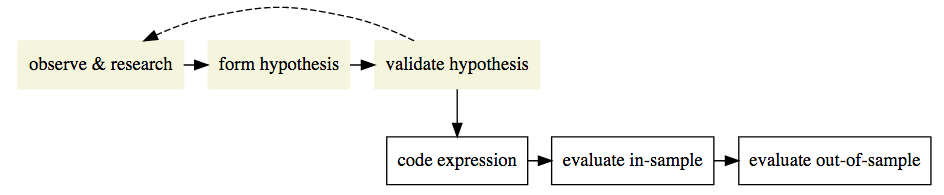
\includegraphics{images/alpha_steps.png}
\caption{image}
\end{figure}

In this project, we assume that the first three steps area done
(``observe \& research'', ``form hypothesis'', ``validate hypothesis'').
The hypothesis you'll be using for this project is the following: - In
the absence of news or significant investor trading interest, stocks
oscillate in a range. - Traders seek to capitalize on this range-bound
behaviour periodically by selling/shorting at the top of the range and
buying/covering at the bottom of the range. This behaviour reinforces
the existence of the range. - When stocks break out of the range, due
to, e.g., a significant news release or from market pressure from a
large investor: - the liquidity traders who have been providing
liquidity at the bounds of the range seek to cover their positions to
mitigate losses, thus magnifying the move out of the range, \emph{and} -
the move out of the range attracts other investor interest; these
investors, due to the behavioural bias of \emph{herding} (e.g.,
\href{https://www.investopedia.com/university/behavioral_finance/behavioral8.asp}{Herd
Behavior}) build positions which favor continuation of the trend.

Using this hypothesis, let start coding.. \#\# Compute the Highs and
Lows in a Window You'll use the price highs and lows as an indicator for
the breakout strategy. In this section, implement
\texttt{get\_high\_lows\_lookback} to get the maximum high price and
minimum low price over a window of days. The variable
\texttt{lookback\_days} contains the number of days to look in the past.
Make sure this doesn't include the current day.

    \begin{Verbatim}[commandchars=\\\{\}]
{\color{incolor}In [{\color{incolor}9}]:} \PY{k}{def} \PY{n+nf}{get\PYZus{}high\PYZus{}lows\PYZus{}lookback}\PY{p}{(}\PY{n}{high}\PY{p}{,} \PY{n}{low}\PY{p}{,} \PY{n}{lookback\PYZus{}days}\PY{p}{)}\PY{p}{:}
            \PY{l+s+sd}{\PYZdq{}\PYZdq{}\PYZdq{}}
        \PY{l+s+sd}{    Get the highs and lows in a lookback window.}
        \PY{l+s+sd}{    }
        \PY{l+s+sd}{    Parameters}
        \PY{l+s+sd}{    \PYZhy{}\PYZhy{}\PYZhy{}\PYZhy{}\PYZhy{}\PYZhy{}\PYZhy{}\PYZhy{}\PYZhy{}\PYZhy{}}
        \PY{l+s+sd}{    high : DataFrame}
        \PY{l+s+sd}{        High price for each ticker and date}
        \PY{l+s+sd}{    low : DataFrame}
        \PY{l+s+sd}{        Low price for each ticker and date}
        \PY{l+s+sd}{    lookback\PYZus{}days : int}
        \PY{l+s+sd}{        The number of days to look back}
        \PY{l+s+sd}{    }
        \PY{l+s+sd}{    Returns}
        \PY{l+s+sd}{    \PYZhy{}\PYZhy{}\PYZhy{}\PYZhy{}\PYZhy{}\PYZhy{}\PYZhy{}}
        \PY{l+s+sd}{    lookback\PYZus{}high : DataFrame}
        \PY{l+s+sd}{        Lookback high price for each ticker and date}
        \PY{l+s+sd}{    lookback\PYZus{}low : DataFrame}
        \PY{l+s+sd}{        Lookback low price for each ticker and date}
        \PY{l+s+sd}{    \PYZdq{}\PYZdq{}\PYZdq{}}
            \PY{c+c1}{\PYZsh{}TODO: Implement function}
            \PY{n}{lookback\PYZus{}high} \PY{o}{=} \PY{n}{high}\PY{o}{.}\PY{n}{shift}\PY{p}{(}\PY{l+m+mi}{1}\PY{p}{)}\PY{o}{.}\PY{n}{rolling}\PY{p}{(}\PY{n}{window}\PY{o}{=}\PY{n}{lookback\PYZus{}days}\PY{p}{)}\PY{o}{.}\PY{n}{max}\PY{p}{(}\PY{p}{)}
            \PY{n}{lookback\PYZus{}low} \PY{o}{=} \PY{n}{low}\PY{o}{.}\PY{n}{shift}\PY{p}{(}\PY{l+m+mi}{1}\PY{p}{)}\PY{o}{.}\PY{n}{rolling}\PY{p}{(}\PY{n}{window}\PY{o}{=}\PY{n}{lookback\PYZus{}days}\PY{p}{)}\PY{o}{.}\PY{n}{min}\PY{p}{(}\PY{p}{)}
            
            \PY{k}{return} \PY{n}{lookback\PYZus{}high}\PY{p}{,} \PY{n}{lookback\PYZus{}low}
        
        \PY{n}{project\PYZus{}tests}\PY{o}{.}\PY{n}{test\PYZus{}get\PYZus{}high\PYZus{}lows\PYZus{}lookback}\PY{p}{(}\PY{n}{get\PYZus{}high\PYZus{}lows\PYZus{}lookback}\PY{p}{)}
\end{Verbatim}


    \begin{Verbatim}[commandchars=\\\{\}]
Tests Passed

    \end{Verbatim}

    \hypertarget{view-data}{%
\subsubsection{View Data}\label{view-data}}

Let's use your implementation of \texttt{get\_high\_lows\_lookback} to
get the highs and lows for the past 50 days and compare it to it their
respective stock. Just like last time, we'll use Apple's stock as the
example to look at.

    \begin{Verbatim}[commandchars=\\\{\}]
{\color{incolor}In [{\color{incolor}10}]:} \PY{n}{lookback\PYZus{}days} \PY{o}{=} \PY{l+m+mi}{50}
         \PY{n}{lookback\PYZus{}high}\PY{p}{,} \PY{n}{lookback\PYZus{}low} \PY{o}{=} \PY{n}{get\PYZus{}high\PYZus{}lows\PYZus{}lookback}\PY{p}{(}\PY{n}{high}\PY{p}{,} \PY{n}{low}\PY{p}{,} \PY{n}{lookback\PYZus{}days}\PY{p}{)}
         \PY{n}{project\PYZus{}helper}\PY{o}{.}\PY{n}{plot\PYZus{}high\PYZus{}low}\PY{p}{(}
             \PY{n}{close}\PY{p}{[}\PY{n}{apple\PYZus{}ticker}\PY{p}{]}\PY{p}{,}
             \PY{n}{lookback\PYZus{}high}\PY{p}{[}\PY{n}{apple\PYZus{}ticker}\PY{p}{]}\PY{p}{,}
             \PY{n}{lookback\PYZus{}low}\PY{p}{[}\PY{n}{apple\PYZus{}ticker}\PY{p}{]}\PY{p}{,}
             \PY{l+s+s1}{\PYZsq{}}\PY{l+s+s1}{High and Low of }\PY{l+s+si}{\PYZob{}\PYZcb{}}\PY{l+s+s1}{ Stock}\PY{l+s+s1}{\PYZsq{}}\PY{o}{.}\PY{n}{format}\PY{p}{(}\PY{n}{apple\PYZus{}ticker}\PY{p}{)}\PY{p}{)}
\end{Verbatim}


    
    
    \hypertarget{compute-long-and-short-signals}{%
\subsection{Compute Long and Short
Signals}\label{compute-long-and-short-signals}}

Using the generated indicator of highs and lows, create long and short
signals using a breakout strategy. Implement \texttt{get\_long\_short}
to generate the following signals:

\begin{longtable}[]{@{}ll@{}}
\toprule
Signal & Condition\tabularnewline
\midrule
\endhead
-1 & Low \textgreater{} Close Price\tabularnewline
1 & High \textless{} Close Price\tabularnewline
0 & Otherwise\tabularnewline
\bottomrule
\end{longtable}

In this chart, \textbf{Close Price} is the \texttt{close} parameter.
\textbf{Low} and \textbf{High} are the values generated from
\texttt{get\_high\_lows\_lookback}, the \texttt{lookback\_high} and
\texttt{lookback\_low} parameters.

    \begin{Verbatim}[commandchars=\\\{\}]
{\color{incolor}In [{\color{incolor}17}]:} \PY{k}{def} \PY{n+nf}{get\PYZus{}long\PYZus{}short}\PY{p}{(}\PY{n}{close}\PY{p}{,} \PY{n}{lookback\PYZus{}high}\PY{p}{,} \PY{n}{lookback\PYZus{}low}\PY{p}{)}\PY{p}{:}
             \PY{l+s+sd}{\PYZdq{}\PYZdq{}\PYZdq{}}
         \PY{l+s+sd}{    Generate the signals long, short, and do nothing.}
         \PY{l+s+sd}{    }
         \PY{l+s+sd}{    Parameters}
         \PY{l+s+sd}{    \PYZhy{}\PYZhy{}\PYZhy{}\PYZhy{}\PYZhy{}\PYZhy{}\PYZhy{}\PYZhy{}\PYZhy{}\PYZhy{}}
         \PY{l+s+sd}{    close : DataFrame}
         \PY{l+s+sd}{        Close price for each ticker and date}
         \PY{l+s+sd}{    lookback\PYZus{}high : DataFrame}
         \PY{l+s+sd}{        Lookback high price for each ticker and date}
         \PY{l+s+sd}{    lookback\PYZus{}low : DataFrame}
         \PY{l+s+sd}{        Lookback low price for each ticker and date}
         \PY{l+s+sd}{    }
         \PY{l+s+sd}{    Returns}
         \PY{l+s+sd}{    \PYZhy{}\PYZhy{}\PYZhy{}\PYZhy{}\PYZhy{}\PYZhy{}\PYZhy{}}
         \PY{l+s+sd}{    long\PYZus{}short : DataFrame}
         \PY{l+s+sd}{        The long, short, and do nothing signals for each ticker and date}
         \PY{l+s+sd}{    \PYZdq{}\PYZdq{}\PYZdq{}}
             \PY{c+c1}{\PYZsh{}TODO: Implement function}
             \PY{n}{long\PYZus{}signals} \PY{o}{=} \PY{p}{(}\PY{n}{close} \PY{o}{\PYZgt{}} \PY{n}{lookback\PYZus{}high}\PY{p}{)}\PY{o}{.}\PY{n}{astype}\PY{p}{(}\PY{n}{np}\PY{o}{.}\PY{n}{int}\PY{p}{)}
             \PY{n}{short\PYZus{}signals} \PY{o}{=} \PY{p}{(}\PY{n}{close} \PY{o}{\PYZlt{}} \PY{n}{lookback\PYZus{}low}\PY{p}{)}\PY{o}{.}\PY{n}{astype}\PY{p}{(}\PY{n}{np}\PY{o}{.}\PY{n}{int}\PY{p}{)} \PY{o}{*} \PY{o}{\PYZhy{}}\PY{l+m+mi}{1}
             \PY{n}{long\PYZus{}short} \PY{o}{=} \PY{n}{long\PYZus{}signals} \PY{o}{+} \PY{n}{short\PYZus{}signals}
             
             \PY{k}{return} \PY{n}{long\PYZus{}short}
         
         \PY{n}{project\PYZus{}tests}\PY{o}{.}\PY{n}{test\PYZus{}get\PYZus{}long\PYZus{}short}\PY{p}{(}\PY{n}{get\PYZus{}long\PYZus{}short}\PY{p}{)}
\end{Verbatim}


    \begin{Verbatim}[commandchars=\\\{\}]
Tests Passed

    \end{Verbatim}

    \hypertarget{view-data}{%
\subsubsection{View Data}\label{view-data}}

Let's compare the signals you generated against the close prices. This
chart will show a lot of signals. Too many in fact. We'll talk about
filtering the redundant signals in the next problem.

    \begin{Verbatim}[commandchars=\\\{\}]
{\color{incolor}In [{\color{incolor}16}]:} \PY{n}{signal} \PY{o}{=} \PY{n}{get\PYZus{}long\PYZus{}short}\PY{p}{(}\PY{n}{close}\PY{p}{,} \PY{n}{lookback\PYZus{}high}\PY{p}{,} \PY{n}{lookback\PYZus{}low}\PY{p}{)}
         \PY{n}{project\PYZus{}helper}\PY{o}{.}\PY{n}{plot\PYZus{}signal}\PY{p}{(}
             \PY{n}{close}\PY{p}{[}\PY{n}{apple\PYZus{}ticker}\PY{p}{]}\PY{p}{,}
             \PY{n}{signal}\PY{p}{[}\PY{n}{apple\PYZus{}ticker}\PY{p}{]}\PY{p}{,}
             \PY{l+s+s1}{\PYZsq{}}\PY{l+s+s1}{Long and Short of }\PY{l+s+si}{\PYZob{}\PYZcb{}}\PY{l+s+s1}{ Stock}\PY{l+s+s1}{\PYZsq{}}\PY{o}{.}\PY{n}{format}\PY{p}{(}\PY{n}{apple\PYZus{}ticker}\PY{p}{)}\PY{p}{)}
\end{Verbatim}


    
    
    \hypertarget{filter-signals}{%
\subsection{Filter Signals}\label{filter-signals}}

That was a lot of repeated signals! If we're already shorting a stock,
having an additional signal to short a stock isn't helpful for this
strategy. This also applies to additional long signals when the last
signal was long.

Implement \texttt{filter\_signals} to filter out repeated long or short
signals within the \texttt{lookahead\_days}. If the previous signal was
the same, change the signal to \texttt{0} (do nothing signal). For
example, say you have a single stock time series that is

\texttt{{[}1,\ 0,\ 1,\ 0,\ 1,\ 0,\ -1,\ -1{]}}

Running \texttt{filter\_signals} with a lookahead of 3 days should turn
those signals into

\texttt{{[}1,\ 0,\ 0,\ 0,\ 1,\ 0,\ -1,\ 0{]}}

To help you implement the function, we have provided you with the
\texttt{clear\_signals} function. This will remove all signals within a
window after the last signal. For example, say you're using a windows
size of 3 with \texttt{clear\_signals}. It would turn the Series of long
signals

\texttt{{[}0,\ 1,\ 0,\ 0,\ 1,\ 1,\ 0,\ 1,\ 0{]}}

into

\texttt{{[}0,\ 1,\ 0,\ 0,\ 0,\ 1,\ 0,\ 0,\ 0{]}}

\texttt{clear\_signals} only takes a Series of the same type of signals,
where \texttt{1} is the signal and \texttt{0} is no signal. It can't
take a mix of long and short signals. Using this function, implement
\texttt{filter\_signals}.

For implementing \texttt{filter\_signals}, we don't reccommend you try
to find a vectorized solution. Instead, you should use the
\href{https://pandas.pydata.org/pandas-docs/version/0.21/generated/pandas.DataFrame.iterrows.html}{\texttt{iterrows}}
over each column.

    \begin{Verbatim}[commandchars=\\\{\}]
{\color{incolor}In [{\color{incolor}46}]:} \PY{k}{def} \PY{n+nf}{clear\PYZus{}signals}\PY{p}{(}\PY{n}{signals}\PY{p}{,} \PY{n}{window\PYZus{}size}\PY{p}{)}\PY{p}{:}
             \PY{l+s+sd}{\PYZdq{}\PYZdq{}\PYZdq{}}
         \PY{l+s+sd}{    Clear out signals in a Series of just long or short signals.}
         \PY{l+s+sd}{    }
         \PY{l+s+sd}{    Remove the number of signals down to 1 within the window size time period.}
         \PY{l+s+sd}{    }
         \PY{l+s+sd}{    Parameters}
         \PY{l+s+sd}{    \PYZhy{}\PYZhy{}\PYZhy{}\PYZhy{}\PYZhy{}\PYZhy{}\PYZhy{}\PYZhy{}\PYZhy{}\PYZhy{}}
         \PY{l+s+sd}{    signals : Pandas Series}
         \PY{l+s+sd}{        The long, short, or do nothing signals}
         \PY{l+s+sd}{    window\PYZus{}size : int}
         \PY{l+s+sd}{        The number of days to have a single signal       }
         \PY{l+s+sd}{    }
         \PY{l+s+sd}{    Returns}
         \PY{l+s+sd}{    \PYZhy{}\PYZhy{}\PYZhy{}\PYZhy{}\PYZhy{}\PYZhy{}\PYZhy{}}
         \PY{l+s+sd}{    signals : Pandas Series}
         \PY{l+s+sd}{        Signals with the signals removed from the window size}
         \PY{l+s+sd}{    \PYZdq{}\PYZdq{}\PYZdq{}}
             \PY{c+c1}{\PYZsh{} Start with buffer of window size}
             \PY{c+c1}{\PYZsh{} This handles the edge case of calculating past\PYZus{}signal in the beginning}
             \PY{n}{clean\PYZus{}signals} \PY{o}{=} \PY{p}{[}\PY{l+m+mi}{0}\PY{p}{]}\PY{o}{*}\PY{n}{window\PYZus{}size}
             
             \PY{k}{for} \PY{n}{signal\PYZus{}i}\PY{p}{,} \PY{n}{current\PYZus{}signal} \PY{o+ow}{in} \PY{n+nb}{enumerate}\PY{p}{(}\PY{n}{signals}\PY{p}{)}\PY{p}{:}
                 \PY{c+c1}{\PYZsh{} Check if there was a signal in the past window\PYZus{}size of days}
                 \PY{n}{has\PYZus{}past\PYZus{}signal} \PY{o}{=} \PY{n+nb}{bool}\PY{p}{(}\PY{n+nb}{sum}\PY{p}{(}\PY{n}{clean\PYZus{}signals}\PY{p}{[}\PY{n}{signal\PYZus{}i}\PY{p}{:}\PY{n}{signal\PYZus{}i}\PY{o}{+}\PY{n}{window\PYZus{}size}\PY{p}{]}\PY{p}{)}\PY{p}{)}
                 \PY{c+c1}{\PYZsh{} Use the current signal if there\PYZsq{}s no past signal, else 0/False}
                 \PY{n}{clean\PYZus{}signals}\PY{o}{.}\PY{n}{append}\PY{p}{(}\PY{o+ow}{not} \PY{n}{has\PYZus{}past\PYZus{}signal} \PY{o+ow}{and} \PY{n}{current\PYZus{}signal}\PY{p}{)}
                 
             \PY{c+c1}{\PYZsh{} Remove buffer}
             \PY{n}{clean\PYZus{}signals} \PY{o}{=} \PY{n}{clean\PYZus{}signals}\PY{p}{[}\PY{n}{window\PYZus{}size}\PY{p}{:}\PY{p}{]}
         
             \PY{c+c1}{\PYZsh{} Return the signals as a Series of Ints}
             \PY{k}{return} \PY{n}{pd}\PY{o}{.}\PY{n}{Series}\PY{p}{(}\PY{n}{np}\PY{o}{.}\PY{n}{array}\PY{p}{(}\PY{n}{clean\PYZus{}signals}\PY{p}{)}\PY{o}{.}\PY{n}{astype}\PY{p}{(}\PY{n}{np}\PY{o}{.}\PY{n}{int}\PY{p}{)}\PY{p}{,} \PY{n}{signals}\PY{o}{.}\PY{n}{index}\PY{p}{)}
         
         
         \PY{k}{def} \PY{n+nf}{filter\PYZus{}signals}\PY{p}{(}\PY{n}{signal}\PY{p}{,} \PY{n}{lookahead\PYZus{}days}\PY{p}{)}\PY{p}{:}
             \PY{l+s+sd}{\PYZdq{}\PYZdq{}\PYZdq{}}
         \PY{l+s+sd}{    Filter out signals in a DataFrame.}
         \PY{l+s+sd}{    }
         \PY{l+s+sd}{    Parameters}
         \PY{l+s+sd}{    \PYZhy{}\PYZhy{}\PYZhy{}\PYZhy{}\PYZhy{}\PYZhy{}\PYZhy{}\PYZhy{}\PYZhy{}\PYZhy{}}
         \PY{l+s+sd}{    signal : DataFrame}
         \PY{l+s+sd}{        The long, short, and do nothing signals for each ticker and date}
         \PY{l+s+sd}{    lookahead\PYZus{}days : int}
         \PY{l+s+sd}{        The number of days to look ahead}
         \PY{l+s+sd}{    }
         \PY{l+s+sd}{    Returns}
         \PY{l+s+sd}{    \PYZhy{}\PYZhy{}\PYZhy{}\PYZhy{}\PYZhy{}\PYZhy{}\PYZhy{}}
         \PY{l+s+sd}{    filtered\PYZus{}signal : DataFrame}
         \PY{l+s+sd}{        The filtered long, short, and do nothing signals for each ticker and date}
         \PY{l+s+sd}{    \PYZdq{}\PYZdq{}\PYZdq{}}
             \PY{c+c1}{\PYZsh{}TODO: Implement function}
             \PY{n}{filtered\PYZus{}signal} \PY{o}{=} \PY{n}{signal}\PY{o}{.}\PY{n}{copy}\PY{p}{(}\PY{p}{)}
             
             \PY{n}{long\PYZus{}signals} \PY{o}{=} \PY{n}{np}\PY{o}{.}\PY{n}{floor}\PY{p}{(}\PY{p}{(}\PY{n}{signal} \PY{o}{+} \PY{l+m+mi}{1}\PY{p}{)} \PY{o}{/} \PY{l+m+mi}{2}\PY{p}{)}\PY{o}{.}\PY{n}{astype}\PY{p}{(}\PY{n}{np}\PY{o}{.}\PY{n}{int}\PY{p}{)}
             \PY{n}{short\PYZus{}signals} \PY{o}{=} \PY{n}{np}\PY{o}{.}\PY{n}{ceil}\PY{p}{(}\PY{p}{(}\PY{n}{signal} \PY{o}{\PYZhy{}} \PY{l+m+mi}{1}\PY{p}{)} \PY{o}{/} \PY{l+m+mi}{2}\PY{p}{)}\PY{o}{.}\PY{n}{astype}\PY{p}{(}\PY{n}{np}\PY{o}{.}\PY{n}{int}\PY{p}{)}
             \PY{k}{for} \PY{n}{column} \PY{o+ow}{in} \PY{n}{signal}\PY{o}{.}\PY{n}{iteritems}\PY{p}{(}\PY{p}{)}\PY{p}{:}
                 \PY{n}{ticker} \PY{o}{=} \PY{n}{column}\PY{p}{[}\PY{l+m+mi}{0}\PY{p}{]}
                 \PY{n}{cleared\PYZus{}long\PYZus{}signals} \PY{o}{=} \PY{n}{clear\PYZus{}signals}\PY{p}{(}\PY{n}{long\PYZus{}signals}\PY{o}{.}\PY{n}{loc}\PY{p}{[}\PY{p}{:}\PY{p}{,}\PY{n}{ticker}\PY{p}{]}\PY{p}{,} \PY{n}{lookahead\PYZus{}days}\PY{p}{)}
                 \PY{n}{cleared\PYZus{}short\PYZus{}signals} \PY{o}{=} \PY{n}{clear\PYZus{}signals}\PY{p}{(}\PY{n}{short\PYZus{}signals}\PY{o}{.}\PY{n}{loc}\PY{p}{[}\PY{p}{:}\PY{p}{,}\PY{n}{ticker}\PY{p}{]}\PY{p}{,} \PY{n}{lookahead\PYZus{}days}\PY{p}{)}
                 \PY{n}{filtered\PYZus{}signal}\PY{o}{.}\PY{n}{loc}\PY{p}{[}\PY{p}{:}\PY{p}{,}\PY{n}{ticker}\PY{p}{]} \PY{o}{=} \PY{n}{cleared\PYZus{}long\PYZus{}signals} \PY{o}{+} \PY{n}{cleared\PYZus{}short\PYZus{}signals}
             
             \PY{k}{return} \PY{n}{filtered\PYZus{}signal}
         
         \PY{n}{project\PYZus{}tests}\PY{o}{.}\PY{n}{test\PYZus{}filter\PYZus{}signals}\PY{p}{(}\PY{n}{filter\PYZus{}signals}\PY{p}{)}
\end{Verbatim}


    \begin{Verbatim}[commandchars=\\\{\}]
Tests Passed

    \end{Verbatim}

    \hypertarget{view-data}{%
\subsubsection{View Data}\label{view-data}}

Let's view the same chart as before, but with the redundant signals
removed.

    \begin{Verbatim}[commandchars=\\\{\}]
{\color{incolor}In [{\color{incolor}47}]:} \PY{n}{signal\PYZus{}5} \PY{o}{=} \PY{n}{filter\PYZus{}signals}\PY{p}{(}\PY{n}{signal}\PY{p}{,} \PY{l+m+mi}{5}\PY{p}{)}
         \PY{n}{signal\PYZus{}10} \PY{o}{=} \PY{n}{filter\PYZus{}signals}\PY{p}{(}\PY{n}{signal}\PY{p}{,} \PY{l+m+mi}{10}\PY{p}{)}
         \PY{n}{signal\PYZus{}20} \PY{o}{=} \PY{n}{filter\PYZus{}signals}\PY{p}{(}\PY{n}{signal}\PY{p}{,} \PY{l+m+mi}{20}\PY{p}{)}
         \PY{k}{for} \PY{n}{signal\PYZus{}data}\PY{p}{,} \PY{n}{signal\PYZus{}days} \PY{o+ow}{in} \PY{p}{[}\PY{p}{(}\PY{n}{signal\PYZus{}5}\PY{p}{,} \PY{l+m+mi}{5}\PY{p}{)}\PY{p}{,} \PY{p}{(}\PY{n}{signal\PYZus{}10}\PY{p}{,} \PY{l+m+mi}{10}\PY{p}{)}\PY{p}{,} \PY{p}{(}\PY{n}{signal\PYZus{}20}\PY{p}{,} \PY{l+m+mi}{20}\PY{p}{)}\PY{p}{]}\PY{p}{:}
             \PY{n}{project\PYZus{}helper}\PY{o}{.}\PY{n}{plot\PYZus{}signal}\PY{p}{(}
                 \PY{n}{close}\PY{p}{[}\PY{n}{apple\PYZus{}ticker}\PY{p}{]}\PY{p}{,}
                 \PY{n}{signal\PYZus{}data}\PY{p}{[}\PY{n}{apple\PYZus{}ticker}\PY{p}{]}\PY{p}{,}
                 \PY{l+s+s1}{\PYZsq{}}\PY{l+s+s1}{Long and Short of }\PY{l+s+si}{\PYZob{}\PYZcb{}}\PY{l+s+s1}{ Stock with }\PY{l+s+si}{\PYZob{}\PYZcb{}}\PY{l+s+s1}{ day signal window}\PY{l+s+s1}{\PYZsq{}}\PY{o}{.}\PY{n}{format}\PY{p}{(}\PY{n}{apple\PYZus{}ticker}\PY{p}{,} \PY{n}{signal\PYZus{}days}\PY{p}{)}\PY{p}{)}
\end{Verbatim}


    
    
    
    
    
    
    \hypertarget{lookahead-close-prices}{%
\subsection{Lookahead Close Prices}\label{lookahead-close-prices}}

With the trading signal done, we can start working on evaluating how
many days to short or long the stocks. In this problem, implement
\texttt{get\_lookahead\_prices} to get the close price days ahead in
time. You can get the number of days from the variable
\texttt{lookahead\_days}. We'll use the lookahead prices to calculate
future returns in another problem.

    \begin{Verbatim}[commandchars=\\\{\}]
{\color{incolor}In [{\color{incolor}49}]:} \PY{k}{def} \PY{n+nf}{get\PYZus{}lookahead\PYZus{}prices}\PY{p}{(}\PY{n}{close}\PY{p}{,} \PY{n}{lookahead\PYZus{}days}\PY{p}{)}\PY{p}{:}
             \PY{l+s+sd}{\PYZdq{}\PYZdq{}\PYZdq{}}
         \PY{l+s+sd}{    Get the lookahead prices for `lookahead\PYZus{}days` number of days.}
         \PY{l+s+sd}{    }
         \PY{l+s+sd}{    Parameters}
         \PY{l+s+sd}{    \PYZhy{}\PYZhy{}\PYZhy{}\PYZhy{}\PYZhy{}\PYZhy{}\PYZhy{}\PYZhy{}\PYZhy{}\PYZhy{}}
         \PY{l+s+sd}{    close : DataFrame}
         \PY{l+s+sd}{        Close price for each ticker and date}
         \PY{l+s+sd}{    lookahead\PYZus{}days : int}
         \PY{l+s+sd}{        The number of days to look ahead}
         \PY{l+s+sd}{    }
         \PY{l+s+sd}{    Returns}
         \PY{l+s+sd}{    \PYZhy{}\PYZhy{}\PYZhy{}\PYZhy{}\PYZhy{}\PYZhy{}\PYZhy{}}
         \PY{l+s+sd}{    lookahead\PYZus{}prices : DataFrame}
         \PY{l+s+sd}{        The lookahead prices for each ticker and date}
         \PY{l+s+sd}{    \PYZdq{}\PYZdq{}\PYZdq{}}
             \PY{c+c1}{\PYZsh{}TODO: Implement function}
             
             \PY{k}{return} \PY{n}{close}\PY{o}{.}\PY{n}{shift}\PY{p}{(}\PY{o}{\PYZhy{}}\PY{l+m+mi}{1}\PY{o}{*}\PY{n}{lookahead\PYZus{}days}\PY{p}{)}
         
         \PY{n}{project\PYZus{}tests}\PY{o}{.}\PY{n}{test\PYZus{}get\PYZus{}lookahead\PYZus{}prices}\PY{p}{(}\PY{n}{get\PYZus{}lookahead\PYZus{}prices}\PY{p}{)}
\end{Verbatim}


    \begin{Verbatim}[commandchars=\\\{\}]
Tests Passed

    \end{Verbatim}

    \hypertarget{view-data}{%
\subsubsection{View Data}\label{view-data}}

Using the \texttt{get\_lookahead\_prices} function, let's generate
lookahead closing prices for 5, 10, and 20 days.

Let's also chart a subsection of a few months of the Apple stock instead
of years. This will allow you to view the differences between the 5, 10,
and 20 day lookaheads. Otherwise, they will mesh together when looking
at a chart that is zoomed out.

    \begin{Verbatim}[commandchars=\\\{\}]
{\color{incolor}In [{\color{incolor}50}]:} \PY{n}{lookahead\PYZus{}5} \PY{o}{=} \PY{n}{get\PYZus{}lookahead\PYZus{}prices}\PY{p}{(}\PY{n}{close}\PY{p}{,} \PY{l+m+mi}{5}\PY{p}{)}
         \PY{n}{lookahead\PYZus{}10} \PY{o}{=} \PY{n}{get\PYZus{}lookahead\PYZus{}prices}\PY{p}{(}\PY{n}{close}\PY{p}{,} \PY{l+m+mi}{10}\PY{p}{)}
         \PY{n}{lookahead\PYZus{}20} \PY{o}{=} \PY{n}{get\PYZus{}lookahead\PYZus{}prices}\PY{p}{(}\PY{n}{close}\PY{p}{,} \PY{l+m+mi}{20}\PY{p}{)}
         \PY{n}{project\PYZus{}helper}\PY{o}{.}\PY{n}{plot\PYZus{}lookahead\PYZus{}prices}\PY{p}{(}
             \PY{n}{close}\PY{p}{[}\PY{n}{apple\PYZus{}ticker}\PY{p}{]}\PY{o}{.}\PY{n}{iloc}\PY{p}{[}\PY{l+m+mi}{150}\PY{p}{:}\PY{l+m+mi}{250}\PY{p}{]}\PY{p}{,}
             \PY{p}{[}
                 \PY{p}{(}\PY{n}{lookahead\PYZus{}5}\PY{p}{[}\PY{n}{apple\PYZus{}ticker}\PY{p}{]}\PY{o}{.}\PY{n}{iloc}\PY{p}{[}\PY{l+m+mi}{150}\PY{p}{:}\PY{l+m+mi}{250}\PY{p}{]}\PY{p}{,} \PY{l+m+mi}{5}\PY{p}{)}\PY{p}{,}
                 \PY{p}{(}\PY{n}{lookahead\PYZus{}10}\PY{p}{[}\PY{n}{apple\PYZus{}ticker}\PY{p}{]}\PY{o}{.}\PY{n}{iloc}\PY{p}{[}\PY{l+m+mi}{150}\PY{p}{:}\PY{l+m+mi}{250}\PY{p}{]}\PY{p}{,} \PY{l+m+mi}{10}\PY{p}{)}\PY{p}{,}
                 \PY{p}{(}\PY{n}{lookahead\PYZus{}20}\PY{p}{[}\PY{n}{apple\PYZus{}ticker}\PY{p}{]}\PY{o}{.}\PY{n}{iloc}\PY{p}{[}\PY{l+m+mi}{150}\PY{p}{:}\PY{l+m+mi}{250}\PY{p}{]}\PY{p}{,} \PY{l+m+mi}{20}\PY{p}{)}\PY{p}{]}\PY{p}{,}
             \PY{l+s+s1}{\PYZsq{}}\PY{l+s+s1}{5, 10, and 20 day Lookahead Prices for Slice of }\PY{l+s+si}{\PYZob{}\PYZcb{}}\PY{l+s+s1}{ Stock}\PY{l+s+s1}{\PYZsq{}}\PY{o}{.}\PY{n}{format}\PY{p}{(}\PY{n}{apple\PYZus{}ticker}\PY{p}{)}\PY{p}{)}
\end{Verbatim}


    
    
    \hypertarget{lookahead-price-returns}{%
\subsection{Lookahead Price Returns}\label{lookahead-price-returns}}

Implement \texttt{get\_return\_lookahead} to generate the log price
return between the closing price and the lookahead price.

    \begin{Verbatim}[commandchars=\\\{\}]
{\color{incolor}In [{\color{incolor}52}]:} \PY{k}{def} \PY{n+nf}{get\PYZus{}return\PYZus{}lookahead}\PY{p}{(}\PY{n}{close}\PY{p}{,} \PY{n}{lookahead\PYZus{}prices}\PY{p}{)}\PY{p}{:}
             \PY{l+s+sd}{\PYZdq{}\PYZdq{}\PYZdq{}}
         \PY{l+s+sd}{    Calculate the log returns from the lookahead days to the signal day.}
         \PY{l+s+sd}{    }
         \PY{l+s+sd}{    Parameters}
         \PY{l+s+sd}{    \PYZhy{}\PYZhy{}\PYZhy{}\PYZhy{}\PYZhy{}\PYZhy{}\PYZhy{}\PYZhy{}\PYZhy{}\PYZhy{}}
         \PY{l+s+sd}{    close : DataFrame}
         \PY{l+s+sd}{        Close price for each ticker and date}
         \PY{l+s+sd}{    lookahead\PYZus{}prices : DataFrame}
         \PY{l+s+sd}{        The lookahead prices for each ticker and date}
         \PY{l+s+sd}{    }
         \PY{l+s+sd}{    Returns}
         \PY{l+s+sd}{    \PYZhy{}\PYZhy{}\PYZhy{}\PYZhy{}\PYZhy{}\PYZhy{}\PYZhy{}}
         \PY{l+s+sd}{    lookahead\PYZus{}returns : DataFrame}
         \PY{l+s+sd}{        The lookahead log returns for each ticker and date}
         \PY{l+s+sd}{    \PYZdq{}\PYZdq{}\PYZdq{}}
             \PY{c+c1}{\PYZsh{}TODO: Implement function}
             
             \PY{k}{return} \PY{n}{np}\PY{o}{.}\PY{n}{log}\PY{p}{(}\PY{n}{lookahead\PYZus{}prices}\PY{p}{)} \PY{o}{\PYZhy{}} \PY{n}{np}\PY{o}{.}\PY{n}{log}\PY{p}{(}\PY{n}{close}\PY{p}{)}
         
         \PY{n}{project\PYZus{}tests}\PY{o}{.}\PY{n}{test\PYZus{}get\PYZus{}return\PYZus{}lookahead}\PY{p}{(}\PY{n}{get\PYZus{}return\PYZus{}lookahead}\PY{p}{)}
\end{Verbatim}


    \begin{Verbatim}[commandchars=\\\{\}]
Tests Passed

    \end{Verbatim}

    \hypertarget{view-data}{%
\subsubsection{View Data}\label{view-data}}

Using the same lookahead prices and same subsection of the Apple stock
from the previous problem, we'll view the lookahead returns.

In order to view price returns on the same chart as the stock, a second
y-axis will be added. When viewing this chart, the axis for the price of
the stock will be on the left side, like previous charts. The axis for
price returns will be located on the right side.

    \begin{Verbatim}[commandchars=\\\{\}]
{\color{incolor}In [{\color{incolor}53}]:} \PY{n}{price\PYZus{}return\PYZus{}5} \PY{o}{=} \PY{n}{get\PYZus{}return\PYZus{}lookahead}\PY{p}{(}\PY{n}{close}\PY{p}{,} \PY{n}{lookahead\PYZus{}5}\PY{p}{)}
         \PY{n}{price\PYZus{}return\PYZus{}10} \PY{o}{=} \PY{n}{get\PYZus{}return\PYZus{}lookahead}\PY{p}{(}\PY{n}{close}\PY{p}{,} \PY{n}{lookahead\PYZus{}10}\PY{p}{)}
         \PY{n}{price\PYZus{}return\PYZus{}20} \PY{o}{=} \PY{n}{get\PYZus{}return\PYZus{}lookahead}\PY{p}{(}\PY{n}{close}\PY{p}{,} \PY{n}{lookahead\PYZus{}20}\PY{p}{)}
         \PY{n}{project\PYZus{}helper}\PY{o}{.}\PY{n}{plot\PYZus{}price\PYZus{}returns}\PY{p}{(}
             \PY{n}{close}\PY{p}{[}\PY{n}{apple\PYZus{}ticker}\PY{p}{]}\PY{o}{.}\PY{n}{iloc}\PY{p}{[}\PY{l+m+mi}{150}\PY{p}{:}\PY{l+m+mi}{250}\PY{p}{]}\PY{p}{,}
             \PY{p}{[}
                 \PY{p}{(}\PY{n}{price\PYZus{}return\PYZus{}5}\PY{p}{[}\PY{n}{apple\PYZus{}ticker}\PY{p}{]}\PY{o}{.}\PY{n}{iloc}\PY{p}{[}\PY{l+m+mi}{150}\PY{p}{:}\PY{l+m+mi}{250}\PY{p}{]}\PY{p}{,} \PY{l+m+mi}{5}\PY{p}{)}\PY{p}{,}
                 \PY{p}{(}\PY{n}{price\PYZus{}return\PYZus{}10}\PY{p}{[}\PY{n}{apple\PYZus{}ticker}\PY{p}{]}\PY{o}{.}\PY{n}{iloc}\PY{p}{[}\PY{l+m+mi}{150}\PY{p}{:}\PY{l+m+mi}{250}\PY{p}{]}\PY{p}{,} \PY{l+m+mi}{10}\PY{p}{)}\PY{p}{,}
                 \PY{p}{(}\PY{n}{price\PYZus{}return\PYZus{}20}\PY{p}{[}\PY{n}{apple\PYZus{}ticker}\PY{p}{]}\PY{o}{.}\PY{n}{iloc}\PY{p}{[}\PY{l+m+mi}{150}\PY{p}{:}\PY{l+m+mi}{250}\PY{p}{]}\PY{p}{,} \PY{l+m+mi}{20}\PY{p}{)}\PY{p}{]}\PY{p}{,}
             \PY{l+s+s1}{\PYZsq{}}\PY{l+s+s1}{5, 10, and 20 day Lookahead Returns for Slice }\PY{l+s+si}{\PYZob{}\PYZcb{}}\PY{l+s+s1}{ Stock}\PY{l+s+s1}{\PYZsq{}}\PY{o}{.}\PY{n}{format}\PY{p}{(}\PY{n}{apple\PYZus{}ticker}\PY{p}{)}\PY{p}{)}
\end{Verbatim}


    
    
    \hypertarget{compute-the-signal-return}{%
\subsection{Compute the Signal Return}\label{compute-the-signal-return}}

Using the price returns generate the signal returns.

    \begin{Verbatim}[commandchars=\\\{\}]
{\color{incolor}In [{\color{incolor}54}]:} \PY{k}{def} \PY{n+nf}{get\PYZus{}signal\PYZus{}return}\PY{p}{(}\PY{n}{signal}\PY{p}{,} \PY{n}{lookahead\PYZus{}returns}\PY{p}{)}\PY{p}{:}
             \PY{l+s+sd}{\PYZdq{}\PYZdq{}\PYZdq{}}
         \PY{l+s+sd}{    Compute the signal returns.}
         \PY{l+s+sd}{    }
         \PY{l+s+sd}{    Parameters}
         \PY{l+s+sd}{    \PYZhy{}\PYZhy{}\PYZhy{}\PYZhy{}\PYZhy{}\PYZhy{}\PYZhy{}\PYZhy{}\PYZhy{}\PYZhy{}}
         \PY{l+s+sd}{    signal : DataFrame}
         \PY{l+s+sd}{        The long, short, and do nothing signals for each ticker and date}
         \PY{l+s+sd}{    lookahead\PYZus{}returns : DataFrame}
         \PY{l+s+sd}{        The lookahead log returns for each ticker and date}
         \PY{l+s+sd}{    }
         \PY{l+s+sd}{    Returns}
         \PY{l+s+sd}{    \PYZhy{}\PYZhy{}\PYZhy{}\PYZhy{}\PYZhy{}\PYZhy{}\PYZhy{}}
         \PY{l+s+sd}{    signal\PYZus{}return : DataFrame}
         \PY{l+s+sd}{        Signal returns for each ticker and date}
         \PY{l+s+sd}{    \PYZdq{}\PYZdq{}\PYZdq{}}
             \PY{c+c1}{\PYZsh{}TODO: Implement function}
             
             \PY{k}{return} \PY{n}{signal} \PY{o}{*} \PY{n}{lookahead\PYZus{}returns}
         
         \PY{n}{project\PYZus{}tests}\PY{o}{.}\PY{n}{test\PYZus{}get\PYZus{}signal\PYZus{}return}\PY{p}{(}\PY{n}{get\PYZus{}signal\PYZus{}return}\PY{p}{)}
\end{Verbatim}


    \begin{Verbatim}[commandchars=\\\{\}]
Tests Passed

    \end{Verbatim}

    \hypertarget{view-data}{%
\subsubsection{View Data}\label{view-data}}

Let's continue using the previous lookahead prices to view the signal
returns. Just like before, the axis for the signal returns is on the
right side of the chart.

    \begin{Verbatim}[commandchars=\\\{\}]
{\color{incolor}In [{\color{incolor}55}]:} \PY{n}{title\PYZus{}string} \PY{o}{=} \PY{l+s+s1}{\PYZsq{}}\PY{l+s+si}{\PYZob{}\PYZcb{}}\PY{l+s+s1}{ day LookaheadSignal Returns for }\PY{l+s+si}{\PYZob{}\PYZcb{}}\PY{l+s+s1}{ Stock}\PY{l+s+s1}{\PYZsq{}}
         \PY{n}{signal\PYZus{}return\PYZus{}5} \PY{o}{=} \PY{n}{get\PYZus{}signal\PYZus{}return}\PY{p}{(}\PY{n}{signal\PYZus{}5}\PY{p}{,} \PY{n}{price\PYZus{}return\PYZus{}5}\PY{p}{)}
         \PY{n}{signal\PYZus{}return\PYZus{}10} \PY{o}{=} \PY{n}{get\PYZus{}signal\PYZus{}return}\PY{p}{(}\PY{n}{signal\PYZus{}10}\PY{p}{,} \PY{n}{price\PYZus{}return\PYZus{}10}\PY{p}{)}
         \PY{n}{signal\PYZus{}return\PYZus{}20} \PY{o}{=} \PY{n}{get\PYZus{}signal\PYZus{}return}\PY{p}{(}\PY{n}{signal\PYZus{}20}\PY{p}{,} \PY{n}{price\PYZus{}return\PYZus{}20}\PY{p}{)}
         \PY{n}{project\PYZus{}helper}\PY{o}{.}\PY{n}{plot\PYZus{}signal\PYZus{}returns}\PY{p}{(}
             \PY{n}{close}\PY{p}{[}\PY{n}{apple\PYZus{}ticker}\PY{p}{]}\PY{p}{,}
             \PY{p}{[}
                 \PY{p}{(}\PY{n}{signal\PYZus{}return\PYZus{}5}\PY{p}{[}\PY{n}{apple\PYZus{}ticker}\PY{p}{]}\PY{p}{,} \PY{n}{signal\PYZus{}5}\PY{p}{[}\PY{n}{apple\PYZus{}ticker}\PY{p}{]}\PY{p}{,} \PY{l+m+mi}{5}\PY{p}{)}\PY{p}{,}
                 \PY{p}{(}\PY{n}{signal\PYZus{}return\PYZus{}10}\PY{p}{[}\PY{n}{apple\PYZus{}ticker}\PY{p}{]}\PY{p}{,} \PY{n}{signal\PYZus{}10}\PY{p}{[}\PY{n}{apple\PYZus{}ticker}\PY{p}{]}\PY{p}{,} \PY{l+m+mi}{10}\PY{p}{)}\PY{p}{,}
                 \PY{p}{(}\PY{n}{signal\PYZus{}return\PYZus{}20}\PY{p}{[}\PY{n}{apple\PYZus{}ticker}\PY{p}{]}\PY{p}{,} \PY{n}{signal\PYZus{}20}\PY{p}{[}\PY{n}{apple\PYZus{}ticker}\PY{p}{]}\PY{p}{,} \PY{l+m+mi}{20}\PY{p}{)}\PY{p}{]}\PY{p}{,}
             \PY{p}{[}\PY{n}{title\PYZus{}string}\PY{o}{.}\PY{n}{format}\PY{p}{(}\PY{l+m+mi}{5}\PY{p}{,} \PY{n}{apple\PYZus{}ticker}\PY{p}{)}\PY{p}{,} \PY{n}{title\PYZus{}string}\PY{o}{.}\PY{n}{format}\PY{p}{(}\PY{l+m+mi}{10}\PY{p}{,} \PY{n}{apple\PYZus{}ticker}\PY{p}{)}\PY{p}{,} \PY{n}{title\PYZus{}string}\PY{o}{.}\PY{n}{format}\PY{p}{(}\PY{l+m+mi}{20}\PY{p}{,} \PY{n}{apple\PYZus{}ticker}\PY{p}{)}\PY{p}{]}\PY{p}{)}
\end{Verbatim}


    
    
    
    
    
    
    \hypertarget{test-for-significance}{%
\subsection{Test for Significance}\label{test-for-significance}}

\hypertarget{histogram}{%
\subsubsection{Histogram}\label{histogram}}

Let's plot a histogram of the signal return values.

    \begin{Verbatim}[commandchars=\\\{\}]
{\color{incolor}In [{\color{incolor}56}]:} \PY{n}{project\PYZus{}helper}\PY{o}{.}\PY{n}{plot\PYZus{}signal\PYZus{}histograms}\PY{p}{(}
             \PY{p}{[}\PY{n}{signal\PYZus{}return\PYZus{}5}\PY{p}{,} \PY{n}{signal\PYZus{}return\PYZus{}10}\PY{p}{,} \PY{n}{signal\PYZus{}return\PYZus{}20}\PY{p}{]}\PY{p}{,}
             \PY{l+s+s1}{\PYZsq{}}\PY{l+s+s1}{Signal Return}\PY{l+s+s1}{\PYZsq{}}\PY{p}{,}
             \PY{p}{(}\PY{l+s+s1}{\PYZsq{}}\PY{l+s+s1}{5 Days}\PY{l+s+s1}{\PYZsq{}}\PY{p}{,} \PY{l+s+s1}{\PYZsq{}}\PY{l+s+s1}{10 Days}\PY{l+s+s1}{\PYZsq{}}\PY{p}{,} \PY{l+s+s1}{\PYZsq{}}\PY{l+s+s1}{20 Days}\PY{l+s+s1}{\PYZsq{}}\PY{p}{)}\PY{p}{)}
\end{Verbatim}


    
    
    \hypertarget{question-what-do-the-histograms-tell-you-about-the-signal-returns}{%
\subsubsection{Question: What do the histograms tell you about the
signal
returns?}\label{question-what-do-the-histograms-tell-you-about-the-signal-returns}}

    \emph{\#TODO: Put Answer In this Cell}

Although the distribution for the 5 day lookahead window more or less
follows the shape of a normal distirbution, as the size of the lookahead
window increases to 10 days, and then to 20 days, there are an
increasing number of stocks giving larger than expected returns. This is
particularly evident in the ``lump'' that can be seen at a return size
of around +0.25 in the `20 day' histogram, giving the graph a shape that
clearly deviates from a normal distribution.

    \hypertarget{outliers}{%
\subsection{Outliers}\label{outliers}}

You might have noticed the outliers in the 10 and 20 day histograms. To
better visualize the outliers, let's compare the 5, 10, and 20 day
signals returns to normal distributions with the same mean and deviation
for each signal return distributions.

    \begin{Verbatim}[commandchars=\\\{\}]
{\color{incolor}In [{\color{incolor}57}]:} \PY{n}{project\PYZus{}helper}\PY{o}{.}\PY{n}{plot\PYZus{}signal\PYZus{}to\PYZus{}normal\PYZus{}histograms}\PY{p}{(}
             \PY{p}{[}\PY{n}{signal\PYZus{}return\PYZus{}5}\PY{p}{,} \PY{n}{signal\PYZus{}return\PYZus{}10}\PY{p}{,} \PY{n}{signal\PYZus{}return\PYZus{}20}\PY{p}{]}\PY{p}{,}
             \PY{l+s+s1}{\PYZsq{}}\PY{l+s+s1}{Signal Return}\PY{l+s+s1}{\PYZsq{}}\PY{p}{,}
             \PY{p}{(}\PY{l+s+s1}{\PYZsq{}}\PY{l+s+s1}{5 Days}\PY{l+s+s1}{\PYZsq{}}\PY{p}{,} \PY{l+s+s1}{\PYZsq{}}\PY{l+s+s1}{10 Days}\PY{l+s+s1}{\PYZsq{}}\PY{p}{,} \PY{l+s+s1}{\PYZsq{}}\PY{l+s+s1}{20 Days}\PY{l+s+s1}{\PYZsq{}}\PY{p}{)}\PY{p}{)}
\end{Verbatim}


    
    
    \hypertarget{kolmogorov-smirnov-test}{%
\subsection{Kolmogorov-Smirnov Test}\label{kolmogorov-smirnov-test}}

While you can see the outliers in the histogram, we need to find the
stocks that are causing these outlying returns. We'll use the
Kolmogorov-Smirnov Test or KS-Test. This test will be applied to teach
ticker's signal returns where a long or short signal exists.

    \begin{Verbatim}[commandchars=\\\{\}]
{\color{incolor}In [{\color{incolor}58}]:} \PY{c+c1}{\PYZsh{} Filter out returns that don\PYZsq{}t have a long or short signal.}
         \PY{n}{long\PYZus{}short\PYZus{}signal\PYZus{}returns\PYZus{}5} \PY{o}{=} \PY{n}{signal\PYZus{}return\PYZus{}5}\PY{p}{[}\PY{n}{signal\PYZus{}5} \PY{o}{!=} \PY{l+m+mi}{0}\PY{p}{]}\PY{o}{.}\PY{n}{stack}\PY{p}{(}\PY{p}{)}
         \PY{n}{long\PYZus{}short\PYZus{}signal\PYZus{}returns\PYZus{}10} \PY{o}{=} \PY{n}{signal\PYZus{}return\PYZus{}10}\PY{p}{[}\PY{n}{signal\PYZus{}10} \PY{o}{!=} \PY{l+m+mi}{0}\PY{p}{]}\PY{o}{.}\PY{n}{stack}\PY{p}{(}\PY{p}{)}
         \PY{n}{long\PYZus{}short\PYZus{}signal\PYZus{}returns\PYZus{}20} \PY{o}{=} \PY{n}{signal\PYZus{}return\PYZus{}20}\PY{p}{[}\PY{n}{signal\PYZus{}20} \PY{o}{!=} \PY{l+m+mi}{0}\PY{p}{]}\PY{o}{.}\PY{n}{stack}\PY{p}{(}\PY{p}{)}
         
         \PY{c+c1}{\PYZsh{} Get just ticker and signal return}
         \PY{n}{long\PYZus{}short\PYZus{}signal\PYZus{}returns\PYZus{}5} \PY{o}{=} \PY{n}{long\PYZus{}short\PYZus{}signal\PYZus{}returns\PYZus{}5}\PY{o}{.}\PY{n}{reset\PYZus{}index}\PY{p}{(}\PY{p}{)}\PY{o}{.}\PY{n}{iloc}\PY{p}{[}\PY{p}{:}\PY{p}{,} \PY{p}{[}\PY{l+m+mi}{1}\PY{p}{,}\PY{l+m+mi}{2}\PY{p}{]}\PY{p}{]}
         \PY{n}{long\PYZus{}short\PYZus{}signal\PYZus{}returns\PYZus{}5}\PY{o}{.}\PY{n}{columns} \PY{o}{=} \PY{p}{[}\PY{l+s+s1}{\PYZsq{}}\PY{l+s+s1}{ticker}\PY{l+s+s1}{\PYZsq{}}\PY{p}{,} \PY{l+s+s1}{\PYZsq{}}\PY{l+s+s1}{signal\PYZus{}return}\PY{l+s+s1}{\PYZsq{}}\PY{p}{]}
         \PY{n}{long\PYZus{}short\PYZus{}signal\PYZus{}returns\PYZus{}10} \PY{o}{=} \PY{n}{long\PYZus{}short\PYZus{}signal\PYZus{}returns\PYZus{}10}\PY{o}{.}\PY{n}{reset\PYZus{}index}\PY{p}{(}\PY{p}{)}\PY{o}{.}\PY{n}{iloc}\PY{p}{[}\PY{p}{:}\PY{p}{,} \PY{p}{[}\PY{l+m+mi}{1}\PY{p}{,}\PY{l+m+mi}{2}\PY{p}{]}\PY{p}{]}
         \PY{n}{long\PYZus{}short\PYZus{}signal\PYZus{}returns\PYZus{}10}\PY{o}{.}\PY{n}{columns} \PY{o}{=} \PY{p}{[}\PY{l+s+s1}{\PYZsq{}}\PY{l+s+s1}{ticker}\PY{l+s+s1}{\PYZsq{}}\PY{p}{,} \PY{l+s+s1}{\PYZsq{}}\PY{l+s+s1}{signal\PYZus{}return}\PY{l+s+s1}{\PYZsq{}}\PY{p}{]}
         \PY{n}{long\PYZus{}short\PYZus{}signal\PYZus{}returns\PYZus{}20} \PY{o}{=} \PY{n}{long\PYZus{}short\PYZus{}signal\PYZus{}returns\PYZus{}20}\PY{o}{.}\PY{n}{reset\PYZus{}index}\PY{p}{(}\PY{p}{)}\PY{o}{.}\PY{n}{iloc}\PY{p}{[}\PY{p}{:}\PY{p}{,} \PY{p}{[}\PY{l+m+mi}{1}\PY{p}{,}\PY{l+m+mi}{2}\PY{p}{]}\PY{p}{]}
         \PY{n}{long\PYZus{}short\PYZus{}signal\PYZus{}returns\PYZus{}20}\PY{o}{.}\PY{n}{columns} \PY{o}{=} \PY{p}{[}\PY{l+s+s1}{\PYZsq{}}\PY{l+s+s1}{ticker}\PY{l+s+s1}{\PYZsq{}}\PY{p}{,} \PY{l+s+s1}{\PYZsq{}}\PY{l+s+s1}{signal\PYZus{}return}\PY{l+s+s1}{\PYZsq{}}\PY{p}{]}
         
         \PY{c+c1}{\PYZsh{} View some of the data}
         \PY{n}{long\PYZus{}short\PYZus{}signal\PYZus{}returns\PYZus{}5}\PY{o}{.}\PY{n}{head}\PY{p}{(}\PY{l+m+mi}{10}\PY{p}{)}
\end{Verbatim}


\begin{Verbatim}[commandchars=\\\{\}]
{\color{outcolor}Out[{\color{outcolor}58}]:}    ticker  signal\_return
         0       A     0.00732604
         1     ABC     0.01639650
         2     ADP     0.00981520
         3  AGENEN     0.01387319
         4    AKAM     0.04400495
         5    ALGN     0.01545561
         6     APC     0.00305859
         7      BA     0.08061297
         8     BCR     0.00933418
         9    BIIB     0.04176183
\end{Verbatim}
            
    This gives you the data to use in the KS-Test.

Now it's time to implement the function \texttt{calculate\_kstest} to
use Kolmogorov-Smirnov test (KS test) between a normal distribution and
each stock's signal returns. Run KS test on a normal distribution
against each stock's signal returns. Use
\href{https://docs.scipy.org/doc/scipy-0.14.0/reference/generated/scipy.stats.kstest.html\#scipy-stats-kstest}{\texttt{scipy.stats.kstest}}
perform the KS test. When calculating the standard deviation of the
signal returns, make sure to set the delta degrees of freedom to 0.

For this function, we don't reccommend you try to find a vectorized
solution. Instead, you should iterate over the
\href{https://pandas.pydata.org/pandas-docs/version/0.21/generated/pandas.DataFrame.groupby.html}{\texttt{groupby}}
function.

    \begin{Verbatim}[commandchars=\\\{\}]
{\color{incolor}In [{\color{incolor}114}]:} \PY{k+kn}{from} \PY{n+nn}{scipy}\PY{n+nn}{.}\PY{n+nn}{stats} \PY{k}{import} \PY{n}{kstest}
          
          
          \PY{k}{def} \PY{n+nf}{calculate\PYZus{}kstest}\PY{p}{(}\PY{n}{long\PYZus{}short\PYZus{}signal\PYZus{}returns}\PY{p}{)}\PY{p}{:}
              \PY{l+s+sd}{\PYZdq{}\PYZdq{}\PYZdq{}}
          \PY{l+s+sd}{    Calculate the KS\PYZhy{}Test against the signal returns with a long or short signal.}
          \PY{l+s+sd}{    }
          \PY{l+s+sd}{    Parameters}
          \PY{l+s+sd}{    \PYZhy{}\PYZhy{}\PYZhy{}\PYZhy{}\PYZhy{}\PYZhy{}\PYZhy{}\PYZhy{}\PYZhy{}\PYZhy{}}
          \PY{l+s+sd}{    long\PYZus{}short\PYZus{}signal\PYZus{}returns : DataFrame}
          \PY{l+s+sd}{        The signal returns which have a signal.}
          \PY{l+s+sd}{        This DataFrame contains two columns, \PYZdq{}ticker\PYZdq{} and \PYZdq{}signal\PYZus{}return\PYZdq{}}
          \PY{l+s+sd}{    }
          \PY{l+s+sd}{    Returns}
          \PY{l+s+sd}{    \PYZhy{}\PYZhy{}\PYZhy{}\PYZhy{}\PYZhy{}\PYZhy{}\PYZhy{}}
          \PY{l+s+sd}{    ks\PYZus{}values : Pandas Series}
          \PY{l+s+sd}{        KS static for all the tickers}
          \PY{l+s+sd}{    p\PYZus{}values : Pandas Series}
          \PY{l+s+sd}{        P value for all the tickers}
          \PY{l+s+sd}{    \PYZdq{}\PYZdq{}\PYZdq{}}
              
              \PY{c+c1}{\PYZsh{}TODO: Implement function}
              \PY{n}{normal\PYZus{}args} \PY{o}{=} \PY{p}{(}\PY{n}{np}\PY{o}{.}\PY{n}{mean}\PY{p}{(}\PY{n}{long\PYZus{}short\PYZus{}signal\PYZus{}returns}\PY{o}{.}\PY{n}{loc}\PY{p}{[}\PY{p}{:}\PY{p}{,}\PY{l+s+s1}{\PYZsq{}}\PY{l+s+s1}{signal\PYZus{}return}\PY{l+s+s1}{\PYZsq{}}\PY{p}{]}\PY{p}{)}\PY{p}{,} 
                             \PY{n}{np}\PY{o}{.}\PY{n}{std}\PY{p}{(}\PY{n}{long\PYZus{}short\PYZus{}signal\PYZus{}returns}\PY{o}{.}\PY{n}{loc}\PY{p}{[}\PY{p}{:}\PY{p}{,}\PY{l+s+s1}{\PYZsq{}}\PY{l+s+s1}{signal\PYZus{}return}\PY{l+s+s1}{\PYZsq{}}\PY{p}{]}\PY{p}{,} \PY{n}{ddof}\PY{o}{=}\PY{l+m+mi}{0}\PY{p}{)}\PY{p}{)}
              
              \PY{n}{ks\PYZus{}results} \PY{o}{=} \PY{n}{long\PYZus{}short\PYZus{}signal\PYZus{}returns}\PY{o}{.}\PY{n}{groupby}\PY{p}{(}\PY{l+s+s1}{\PYZsq{}}\PY{l+s+s1}{ticker}\PY{l+s+s1}{\PYZsq{}}\PY{p}{)}\PY{o}{.}\PY{n}{agg}\PY{p}{(}\PY{k}{lambda} \PY{n}{x}\PY{p}{:} \PY{n}{kstest}\PY{p}{(}\PY{n}{rvs}\PY{o}{=}\PY{n}{x}\PY{p}{,} \PY{n}{cdf}\PY{o}{=}\PY{l+s+s1}{\PYZsq{}}\PY{l+s+s1}{norm}\PY{l+s+s1}{\PYZsq{}}\PY{p}{,} \PY{n}{args}\PY{o}{=}\PY{n}{normal\PYZus{}args}\PY{p}{)}\PY{p}{)}
              
              \PY{n}{ks\PYZus{}values} \PY{o}{=} \PY{n}{ks\PYZus{}results}\PY{o}{.}\PY{n}{applymap}\PY{p}{(}\PY{k}{lambda} \PY{n}{x}\PY{p}{:} \PY{n}{x}\PY{p}{[}\PY{l+m+mi}{0}\PY{p}{]}\PY{p}{)}
              \PY{n}{ks\PYZus{}values}\PY{o}{.}\PY{n}{columns} \PY{o}{=} \PY{p}{[}\PY{l+s+s1}{\PYZsq{}}\PY{l+s+s1}{ks\PYZus{}values}\PY{l+s+s1}{\PYZsq{}}\PY{p}{]}
              \PY{n}{ks\PYZus{}values} \PY{o}{=} \PY{n}{ks\PYZus{}values}\PY{o}{.}\PY{n}{squeeze}\PY{p}{(}\PY{p}{)}
              
              \PY{n}{p\PYZus{}values} \PY{o}{=} \PY{n}{ks\PYZus{}results}\PY{o}{.}\PY{n}{applymap}\PY{p}{(}\PY{k}{lambda} \PY{n}{x}\PY{p}{:} \PY{n}{x}\PY{p}{[}\PY{l+m+mi}{1}\PY{p}{]}\PY{p}{)}
              \PY{n}{p\PYZus{}values}\PY{o}{.}\PY{n}{columns} \PY{o}{=} \PY{p}{[}\PY{l+s+s1}{\PYZsq{}}\PY{l+s+s1}{p\PYZus{}values}\PY{l+s+s1}{\PYZsq{}}\PY{p}{]}
              \PY{n}{p\PYZus{}values} \PY{o}{=} \PY{n}{p\PYZus{}values}\PY{o}{.}\PY{n}{squeeze}\PY{p}{(}\PY{p}{)}
          
              \PY{k}{return} \PY{n}{ks\PYZus{}values}\PY{p}{,} \PY{n}{p\PYZus{}values}
          
          
          \PY{n}{project\PYZus{}tests}\PY{o}{.}\PY{n}{test\PYZus{}calculate\PYZus{}kstest}\PY{p}{(}\PY{n}{calculate\PYZus{}kstest}\PY{p}{)}
\end{Verbatim}


    \begin{Verbatim}[commandchars=\\\{\}]
Tests Passed

    \end{Verbatim}

    \hypertarget{view-data}{%
\subsubsection{View Data}\label{view-data}}

Using the signal returns we created above, let's calculate the ks and p
values.

    \begin{Verbatim}[commandchars=\\\{\}]
{\color{incolor}In [{\color{incolor}115}]:} \PY{n}{ks\PYZus{}values\PYZus{}5}\PY{p}{,} \PY{n}{p\PYZus{}values\PYZus{}5} \PY{o}{=} \PY{n}{calculate\PYZus{}kstest}\PY{p}{(}\PY{n}{long\PYZus{}short\PYZus{}signal\PYZus{}returns\PYZus{}5}\PY{p}{)}
          \PY{n}{ks\PYZus{}values\PYZus{}10}\PY{p}{,} \PY{n}{p\PYZus{}values\PYZus{}10} \PY{o}{=} \PY{n}{calculate\PYZus{}kstest}\PY{p}{(}\PY{n}{long\PYZus{}short\PYZus{}signal\PYZus{}returns\PYZus{}10}\PY{p}{)}
          \PY{n}{ks\PYZus{}values\PYZus{}20}\PY{p}{,} \PY{n}{p\PYZus{}values\PYZus{}20} \PY{o}{=} \PY{n}{calculate\PYZus{}kstest}\PY{p}{(}\PY{n}{long\PYZus{}short\PYZus{}signal\PYZus{}returns\PYZus{}20}\PY{p}{)}
          
          \PY{n+nb}{print}\PY{p}{(}\PY{l+s+s1}{\PYZsq{}}\PY{l+s+s1}{ks\PYZus{}values\PYZus{}5}\PY{l+s+s1}{\PYZsq{}}\PY{p}{)}
          \PY{n+nb}{print}\PY{p}{(}\PY{n}{ks\PYZus{}values\PYZus{}5}\PY{o}{.}\PY{n}{head}\PY{p}{(}\PY{l+m+mi}{10}\PY{p}{)}\PY{p}{)}
          \PY{n+nb}{print}\PY{p}{(}\PY{l+s+s1}{\PYZsq{}}\PY{l+s+s1}{p\PYZus{}values\PYZus{}5}\PY{l+s+s1}{\PYZsq{}}\PY{p}{)}
          \PY{n+nb}{print}\PY{p}{(}\PY{n}{p\PYZus{}values\PYZus{}5}\PY{o}{.}\PY{n}{head}\PY{p}{(}\PY{l+m+mi}{10}\PY{p}{)}\PY{p}{)}
\end{Verbatim}


    \begin{Verbatim}[commandchars=\\\{\}]
ks\_values\_5
ticker
A      0.17206528
AAL    0.10746277
AAP    0.19688949
AAPL   0.15565329
ABBV   0.16810221
ABC    0.21410658
ABT    0.21367025
ACN    0.28219047
ADBE   0.24265899
ADI    0.19428052
Name: ks\_values, dtype: float64
p\_values\_5
ticker
A      0.18748825
AAL    0.72412744
AAP    0.04514860
AAPL   0.24715656
ABBV   0.24721762
ABC    0.02734519
ABT    0.04840102
ACN    0.00586167
ADBE   0.00913261
ADI    0.09890862
Name: p\_values, dtype: float64

    \end{Verbatim}

    \hypertarget{find-outliers}{%
\subsection{Find Outliers}\label{find-outliers}}

With the ks and p values calculate, let's find which symbols are the
outliers. Implement the \texttt{find\_outliers} function to find the
following outliers: - Symbols that pass the null hypothesis with a
p-value less than \texttt{pvalue\_threshold}. - Symbols that with a KS
value above \texttt{ks\_threshold}.

    \begin{Verbatim}[commandchars=\\\{\}]
{\color{incolor}In [{\color{incolor}136}]:} \PY{k}{def} \PY{n+nf}{find\PYZus{}outliers}\PY{p}{(}\PY{n}{ks\PYZus{}values}\PY{p}{,} \PY{n}{p\PYZus{}values}\PY{p}{,} \PY{n}{ks\PYZus{}threshold}\PY{p}{,} \PY{n}{pvalue\PYZus{}threshold}\PY{o}{=}\PY{l+m+mf}{0.05}\PY{p}{)}\PY{p}{:}
              \PY{l+s+sd}{\PYZdq{}\PYZdq{}\PYZdq{}}
          \PY{l+s+sd}{    Find outlying symbols using KS values and P\PYZhy{}values}
          \PY{l+s+sd}{    }
          \PY{l+s+sd}{    Parameters}
          \PY{l+s+sd}{    \PYZhy{}\PYZhy{}\PYZhy{}\PYZhy{}\PYZhy{}\PYZhy{}\PYZhy{}\PYZhy{}\PYZhy{}\PYZhy{}}
          \PY{l+s+sd}{    ks\PYZus{}values : Pandas Series}
          \PY{l+s+sd}{        KS statistic for all the tickers}
          \PY{l+s+sd}{    p\PYZus{}values : Pandas Series}
          \PY{l+s+sd}{        P value for all the tickers}
          \PY{l+s+sd}{    ks\PYZus{}threshold : float}
          \PY{l+s+sd}{        The threshold for the KS statistic}
          \PY{l+s+sd}{    pvalue\PYZus{}threshold : float}
          \PY{l+s+sd}{        The threshold for the p\PYZhy{}value}
          \PY{l+s+sd}{    }
          \PY{l+s+sd}{    Returns}
          \PY{l+s+sd}{    \PYZhy{}\PYZhy{}\PYZhy{}\PYZhy{}\PYZhy{}\PYZhy{}\PYZhy{}}
          \PY{l+s+sd}{    outliers : set of str}
          \PY{l+s+sd}{        Symbols that are outliers}
          \PY{l+s+sd}{    \PYZdq{}\PYZdq{}\PYZdq{}}
              \PY{c+c1}{\PYZsh{}TODO: Implement function}
              \PY{n}{ks\PYZus{}value\PYZus{}outliers} \PY{o}{=} \PY{n}{ks\PYZus{}values} \PY{o}{\PYZgt{}} \PY{n}{ks\PYZus{}threshold}
              \PY{n}{p\PYZus{}value\PYZus{}outliers} \PY{o}{=} \PY{n}{p\PYZus{}values} \PY{o}{\PYZlt{}} \PY{n}{pvalue\PYZus{}threshold}
              \PY{n}{ks\PYZus{}and\PYZus{}p\PYZus{}value\PYZus{}outliers} \PY{o}{=} \PY{p}{(}\PY{n}{ks\PYZus{}value\PYZus{}outliers} \PY{o}{|} \PY{n}{p\PYZus{}value\PYZus{}outliers}\PY{p}{)}\PY{o}{.}\PY{n}{where}\PY{p}{(}\PY{k}{lambda} \PY{n}{x}\PY{p}{:} \PY{n}{x} \PY{o}{==} \PY{k+kc}{True}\PY{p}{)}\PY{o}{.}\PY{n}{dropna}\PY{p}{(}\PY{p}{)}
              \PY{n}{outliers} \PY{o}{=} \PY{n+nb}{set}\PY{p}{(}\PY{n}{ks\PYZus{}and\PYZus{}p\PYZus{}value\PYZus{}outliers}\PY{o}{.}\PY{n}{index}\PY{o}{.}\PY{n}{values}\PY{p}{)}
          
              \PY{k}{return} \PY{n}{outliers}
          
          
          \PY{n}{project\PYZus{}tests}\PY{o}{.}\PY{n}{test\PYZus{}find\PYZus{}outliers}\PY{p}{(}\PY{n}{find\PYZus{}outliers}\PY{p}{)}
\end{Verbatim}


    \begin{Verbatim}[commandchars=\\\{\}]
Tests Passed

    \end{Verbatim}

    \hypertarget{view-data}{%
\subsubsection{View Data}\label{view-data}}

Using the \texttt{find\_outliers} function you implemented, let's see
what we found.

    \begin{Verbatim}[commandchars=\\\{\}]
{\color{incolor}In [{\color{incolor}137}]:} \PY{n}{ks\PYZus{}threshold} \PY{o}{=} \PY{l+m+mf}{0.8}
          \PY{n}{outliers\PYZus{}5} \PY{o}{=} \PY{n}{find\PYZus{}outliers}\PY{p}{(}\PY{n}{ks\PYZus{}values\PYZus{}5}\PY{p}{,} \PY{n}{p\PYZus{}values\PYZus{}5}\PY{p}{,} \PY{n}{ks\PYZus{}threshold}\PY{p}{)}
          \PY{n}{outliers\PYZus{}10} \PY{o}{=} \PY{n}{find\PYZus{}outliers}\PY{p}{(}\PY{n}{ks\PYZus{}values\PYZus{}10}\PY{p}{,} \PY{n}{p\PYZus{}values\PYZus{}10}\PY{p}{,} \PY{n}{ks\PYZus{}threshold}\PY{p}{)}
          \PY{n}{outliers\PYZus{}20} \PY{o}{=} \PY{n}{find\PYZus{}outliers}\PY{p}{(}\PY{n}{ks\PYZus{}values\PYZus{}20}\PY{p}{,} \PY{n}{p\PYZus{}values\PYZus{}20}\PY{p}{,} \PY{n}{ks\PYZus{}threshold}\PY{p}{)}
          
          \PY{n}{outlier\PYZus{}tickers} \PY{o}{=} \PY{n}{outliers\PYZus{}5}\PY{o}{.}\PY{n}{union}\PY{p}{(}\PY{n}{outliers\PYZus{}10}\PY{p}{)}\PY{o}{.}\PY{n}{union}\PY{p}{(}\PY{n}{outliers\PYZus{}20}\PY{p}{)}
          \PY{n+nb}{print}\PY{p}{(}\PY{l+s+s1}{\PYZsq{}}\PY{l+s+si}{\PYZob{}\PYZcb{}}\PY{l+s+s1}{ Outliers Found:}\PY{l+s+se}{\PYZbs{}n}\PY{l+s+si}{\PYZob{}\PYZcb{}}\PY{l+s+s1}{\PYZsq{}}\PY{o}{.}\PY{n}{format}\PY{p}{(}\PY{n+nb}{len}\PY{p}{(}\PY{n}{outlier\PYZus{}tickers}\PY{p}{)}\PY{p}{,} \PY{l+s+s1}{\PYZsq{}}\PY{l+s+s1}{, }\PY{l+s+s1}{\PYZsq{}}\PY{o}{.}\PY{n}{join}\PY{p}{(}\PY{n+nb}{list}\PY{p}{(}\PY{n}{outlier\PYZus{}tickers}\PY{p}{)}\PY{p}{)}\PY{p}{)}\PY{p}{)}
\end{Verbatim}


    \begin{Verbatim}[commandchars=\\\{\}]
300 Outliers Found:
MDLZ, CMCSA, FOX, BMY, ARMENA, EXPE, K, SYLVES, HAS, INCY, GE, PEG, AWK, VFC, GOOGL, CNC, NI, XYL, FE, EL, ACN, AOS, RE, ZBH, MKC, AIG, GM, SAXATI, RJF, LVLT, LMT, RSG, WMT, UAA, WY, FLR, DISCA, SEE, ESRX, JPM, CVS, TMO, GESNER, ABT, PNR, NWL, CHD, APH, CCI, SCHW, T, TURKES, FRT, HCA, AZO, SYY, ADP, ADBE, DTE, UNP, ED, AON, PX, HOLX, KOLPAK, NLSN, PCAR, CTAS, DOV, DPS, AGENEN, PFE, ICE, OXY, AMT, JBHT, MCHP, COL, HON, AJG, GGP, SNA, HRB, GIS, CL, KMX, SRCL, SHW, EQR, SWK, HCN, ALXN, FBHS, XEL, MON, DUK, NSC, XRAY, KHC, CME, OMC, LNC, TAP, WFC, FCX, BAKERI, LINIFO, SYK, MDT, HSY, GWW, ABBV, DG, PBCT, MPC, CRM, TROW, REG, PNC, AIV, SJM, CAG, STZ, ANSS, ABC, AAP, IFF, CSCO, PGR, CBOE, BXP, PEP, UNM, AVB, EQIX, HSIC, ES, ORLY, ESS, MMC, PPL, DIS, LH, HLT, PH, VZ, HRL, DFS, SPRENG, EMN, BIIB, ANTM, PG, KAUFMA, HPE, BDX, ORCL, PLD, FIS, USB, INTU, PULCHE, XOM, HST, BIFLOR, LB, VRTX, KO, ORPHAN, AME, NEM, CAT, CMI, PRAEST, ALTAIC, DASYST, UDR, WAT, MO, QRVO, WU, CHK, VAR, RTN, XRX, PHM, KR, FISV, VNO, AAL, BEN, CNP, FOXA, DGX, NKE, DRE, MS, STT, HUMILI, NOC, IRM, AEP, UNH, CAH, V, LEG, D, PCG, BCR, HBI, HD, LKQ, AIZ, AMD, CLX, TARDA, MCO, UPS, CLUSIA, EMR, VTR, SCG, LNT, GLW, GREIGI, UHS, AMGN, HOG, AMAT, VVEDEN, CI, ROK, ALLE, SRE, ETN, IVZ, HBAN, L, LLY, MAC, MCD, SBUX, BLL, DISCK, SNI, PKG, TDG, TRV, MSFT, FAST, FLIR, MSI, CMS, SO, URUMIE, NWSA, ECL, COST, WM, AFL, EIX, DHR, LOW, SCHREN, ISRG, KLAC, GD, KMB, ROP, NEE, CBS, TMK, TEL, EXC, PSA, DE, HRS, ITW, BAX, MRK, CHTR, ALL, WEC, TSS, PNW, CB, AEE, PDCO, XL, ADS, JNJ, CINF, CA, MTB, TXN, IPG, CPB, GPC, EFX, TJX

    \end{Verbatim}

    \hypertarget{show-significance-without-outliers}{%
\subsubsection{Show Significance without
Outliers}\label{show-significance-without-outliers}}

Let's compare the 5, 10, and 20 day signals returns without outliers to
normal distributions. Also, let's see how the P-Value has changed with
the outliers removed.

    \begin{Verbatim}[commandchars=\\\{\}]
{\color{incolor}In [{\color{incolor}138}]:} \PY{n}{good\PYZus{}tickers} \PY{o}{=} \PY{n+nb}{list}\PY{p}{(}\PY{n+nb}{set}\PY{p}{(}\PY{n}{close}\PY{o}{.}\PY{n}{columns}\PY{p}{)} \PY{o}{\PYZhy{}} \PY{n}{outlier\PYZus{}tickers}\PY{p}{)}
          
          \PY{n}{project\PYZus{}helper}\PY{o}{.}\PY{n}{plot\PYZus{}signal\PYZus{}to\PYZus{}normal\PYZus{}histograms}\PY{p}{(}
              \PY{p}{[}\PY{n}{signal\PYZus{}return\PYZus{}5}\PY{p}{[}\PY{n}{good\PYZus{}tickers}\PY{p}{]}\PY{p}{,} \PY{n}{signal\PYZus{}return\PYZus{}10}\PY{p}{[}\PY{n}{good\PYZus{}tickers}\PY{p}{]}\PY{p}{,} \PY{n}{signal\PYZus{}return\PYZus{}20}\PY{p}{[}\PY{n}{good\PYZus{}tickers}\PY{p}{]}\PY{p}{]}\PY{p}{,}
              \PY{l+s+s1}{\PYZsq{}}\PY{l+s+s1}{Signal Return Without Outliers}\PY{l+s+s1}{\PYZsq{}}\PY{p}{,}
              \PY{p}{(}\PY{l+s+s1}{\PYZsq{}}\PY{l+s+s1}{5 Days}\PY{l+s+s1}{\PYZsq{}}\PY{p}{,} \PY{l+s+s1}{\PYZsq{}}\PY{l+s+s1}{10 Days}\PY{l+s+s1}{\PYZsq{}}\PY{p}{,} \PY{l+s+s1}{\PYZsq{}}\PY{l+s+s1}{20 Days}\PY{l+s+s1}{\PYZsq{}}\PY{p}{)}\PY{p}{)}
\end{Verbatim}


    
    
    That's more like it! The returns are closer to a normal distribution.
You have finished the research phase of a Breakout Strategy. You can now
submit your project. \#\# Submission Now that you're done with the
project, it's time to submit it. Click the submit button in the bottom
right. One of our reviewers will give you feedback on your project with
a pass or not passed grade. You can continue to the next section while
you wait for feedback.


    % Add a bibliography block to the postdoc
    
    
    
    \end{document}
